\chapter{ベクトルと座標系}\label{vecterop}
いままでやってきたのは実数に対して実数を返すような関数に関する微分積分学であった.
いまからやるのは,実数に対してベクトルを返したり,ベクトルに対して実数を返す,
もしくはベクトルに対してベクトルを返すような関数に関する微分積分学である.
何やら難しそうに思えるが実はそうでもない.実数のときの微分積分学の考え方がほぼそのまま使えるのだ.
これは,ベクトルの表し方を考えてみればすぐにわかる.早速やってみようといいたいところだが,
まずはベクトルとは何かを考えてみよう.
\section{ベクトルとその表現方法}
\subsection{ベクトルとは何か}
\emph{ベクトル量}\index[widx]{べくとる@ベクトル}
というのは,向きと大きさを持つ量のことだった.
対して,大きさのみを持つ量を\emph{スカラー量}\index[widx]{すからー@スカラー}
というのだった.
スカラー量を表したいときには,その大きさを表す実数を使えばよい.スカラー量とは実数である...という風に表現したくなるのだが,
現実はもう少し複雑である.正確な定義を述べるのはやや面倒なのでこのあたりで逃げておこう.
ただ,実数は大きさしか持たないからスカラー量とみなしていいだろう.

ベクトルとは向きと大きさを持つ量である...とさっき述べたのだが,実はこれもあまり正確な表現ではない.
さきほど実数は大きさしか持たないという話をした.実数を数直線上に図示してみれば,ただの点であり,方向性などない.
しかし,こうは考えられないだろうか? 方向性を持たないただの点であっても,原点とその点を結べば線分ができあがる.
この線分は原点からその実数に対応する点への向きを持つと考える.
いわゆる\emph{有向線分}\index[widx]{ゆうこうせんぶん@有向線分}
というやつである.
そして,実数というのは実はこの有向線分を表していたのだと考える.
いままで点だと思い込んでいたのはこの有向線分の終点だけを眺めて点だと言い張っていたにすぎないというように考えるのだ.
このように考えてみると,実数というものがあたかもベクトルであるかのように考えることができる.
だが,実数はスカラー量であるという主張にも一定の説得力がある.
いったいどっちなのだというのだろうか? ベクトル量でもありスカラー量でもある.
そんな量が存在するとでもいうのだろうか? この疑問は探求心のある読者のために大事に取っておくことにしよう.
とりあえずいまは,ベクトル量とは向きと大きさを持つ量であるというように認識しておくことにする.

\subsection{ベクトルの表記}
ベクトルは向きと大きさを持つのだった.
そんなものをいったいどうやって表したらいいだろうか? 高校まではおそらく矢印で表していたはずだ.
ベクトルの向きを矢印で,そしてベクトルの大きさを矢印の長さで表すのである.
これはベクトルを図示する方法である.記号で表したいときは,スカラー量と区別するために文字の上に矢印を乗せて
$\vec{a}$などというように表すのだった.これは``$a$ベクトル''や``ベクトル$a$''と読む.前者の読み方を使っている人が多い気がする.
この表記法は実に合理的である.
矢印で表されたベクトルを見れば,その向きと大きさがすぐにわかる.
$\vec{a}$という記号を見れば,これが向きと大きさを持ったベクトルだということが直感的にも理解できる.

だが,普通の専門書では$\to$を用いたベクトルの表記はしない.太字の文字を使って$\bm{a}$というように表記するのである.
なお,読み方はまったく同じで``$a$ベクトル''や``ベクトル$a$''と読む.
ちょっと見づらいが,慣れればなかなか美しいものである.なお,手書きで書くときには普通の文字に線を一本入れて二重文字で表記する.
線をどこに入れるかは好みでよい.あまりに見づらくなってしまうようなものだと困るが.人によって線の入れ方はさまざまである.
要は``この量はベクトル量ですよ''ということがわかればよいのである.
普通の文字が$a, \, b, \, c, \, \cdots$で,
ベクトル表記のものが$\bm{a}, \, \bm{b}, \, \bm{c}, \, \cdots$という具合である.
並べてみれば一目瞭然であるが,これを単独で見たときにきちんと判別しなければならない.
この記法を多用していれば自然と慣れてくるだろう.記号法というものは使って初めて身につくのである.

なぜ矢印ではなく太字を使うのだろうか? 少し考えてみよう.高校数学ではベクトルを何に使うかと言われれば,
図形問題を鮮やかに解くのに使われる.そう,まさにベクトルを矢印とまったく同じものとみなしているのである.
このとき使われるベクトルを\emph{幾何ベクトル}\index[widx]{べくとる@ベクトル!きか@幾何---}
という.ベクトルを一種の図形とみなしているのである.

しかし,これからやるのはそんなものではない.ベクトルを微分したり積分したりするのである.
つまり,ベクトルを関数だとみなすのである.
微分積分学は解析学の基礎的な部分を指す.
ベクトル解析という言葉はここからきている.
たしかに,計算した結果を幾何的に解釈することはあるが,あくまでオマケのようなものである.
このときに使われるベクトルは,もはや幾何ベクトルとはほど遠い.
そんな場合に矢印表記をしていては,むしろ誤解を招きかねない.
そこでベクトルを太字で表記する方法を用いるというわけだ.
その要請のもとは線形代数学にあるといってもいいだろう.
数学者はベクトルの概念を抽象化し,ベクトル空間なるものを考案した.
たしかにベースは幾何ベクトルである.しかし,中身は幾何ベクトルよりもはるかに広い概念を内包している.
そのような理論を組み立てるうえで矢印表記のベクトルは邪魔でしかない.
ベクトルを矢印以外の方法で表記するのはもはや必然である.
物理学でもこのあたりの話題を引っ張ってくることがよくある.量子力学なんかではしょっちゅうである.
\footnote{とはいうものの,量子力学ではブラ・ケット記法という
太字表記とはまた違ったベクトルの表記方法を採用していることが多い.}
分野や流儀によって表記や定義が違うというのはよくあることである.
違う分野や流儀に足を踏みいれるときにはまずそのあたりを確かめるとよい.

 \subsection{書体について}
 表記法をやったついでに書体についても触れておこう.
 普通,自然科学の分野では文字を表すときに\emph{イタリック体}と呼ばれる書体を使う.
 本書でも散々使っている書体である.$x, \, y, \, \varphi, \, A, \, B$などである.
イタリック体は,字がちょっと傾いているのが特徴である.手書きでは面倒なので傾けたりすることは普通しない.
 見返してみればほとんどの文字がイタリック体で書かれているはずである.
 
 しかし,それだけではないはずだ.
 傾いていないものがあるはずである.このような書体は\emph{ローマン体},もしくは
 \emph{立体}と呼ばれる.
 その書体は何を表すときに使われているだろうか? 特徴があるはずだ.
 使う場合はいろいろ考えられる.1つは点を表したいときである.$\triangle \mathrm{ABC}$や点$\mathrm{P}$などがある.
 $\triangle \mathrm{ABC}$というのは図形だが,
それを構成する$\mathrm{A}, \, \mathrm{B}, \, \mathrm{C}$は点である.
また,\emph{演算子}\index[widx]{えんざんし@演算子}なるものを表したいときにもローマン体が使われる.
演算子というのは単体で何かを表すというものではなく,何かの前にくっついてそれとペアで意味を持つものである.
正弦関数$\sin$や指数関数$\exp$,あとは微小量を表す$\mathrm{d}$など
だろうか.\footnote{$\mathrm{d}$に関してはイタリック体で書く流儀も多い.}
イタリック体で書いた通常の変数を表す文字と区別しなければ非常に面倒なことになるのがわかるだろう.
他にも,``いつも変わらない普遍的なモノ''や単位を表すのにもローマン体が使われることがある.
なんだかあいまいな気がするが,たとえばNapire数$\mathrm{e}$や虚数単位$\mathrm{i}$,
それに長さの単位である$[ \mathrm{cm} ]$や時間の単位である$[ \mathrm{s} ]$などである.
ベクトルを表すのにもローマン体が使われることがある.
太字とローマン体とを組み合わせて$\mathbf{x}$や$\mathbf{E}$というように表すのである.
他の本を読むときにはこの点には気を付けていただきたい.
ただし,見栄えが悪くなるので本書ではベクトルはイタリック体の太字で書かせてもらう.
もちろん,ここで書いたのはあくまでそういう傾向があるというだけであり,
そういう風に表記しなければならないと言っているわけではないということに気を付けてもらいたい.
本書でもNapire数$e$や虚数単位$i$などはイタリック体で表記している.
また,本書では原則として演算子と点,そして単位のみをローマン体とし,
他はイタリック体で表記することにする.
もちろんこのような表記法が世界共通というわけではない.
ただし,一度その流儀を採用すると決めたら,それを途中で変えるのは厳禁である.理由は言わなくてもわかるだろう.
無用な混乱は避けるべきである.

表記法に関してはこんなものだろうか.割とみんな好き勝手にやっているのが伝わってくれればそれでいい.

\subsection{数ベクトル空間}
ベクトルを微分したり積分したりしたければ,やっぱり関数が必要である.そのために,ベクトルの成分表示というものを考える.

3次元空間内にベクトル$\bm{a}$がある状況を考える.ベクトルには向きと大きさがある.ベクトルの始点を原点に固定してみよう.
ベクトルには向きと大きさがあるが,それ以外にはなにもない.
向きと大きさを変えないように動かしたところで(これを平行移動という)
やはり同じベクトルである.
ベクトルの始点を原点に固定したとき,その終点が点$(a_1, \, a_2, \, a_3)$であったとする.
いつでもベクトルの始点を原点に固定すると約束しておけば,終点の座標を決めるだけでベクトルを決めることができる.
つまり,終点の座標$(a_1, \,  a_2, \, a_3)$を書いておくだけでこのベクトルがどんなベクトルかわかるのである.
わざわざ矢印など書かなくとも,ただ数を3つ並べるだけでいいのだ.
この便利さを認め,点の座標と区別するために表記をちょっと変えて
\begin{align}
\bm{a} = \left[
 \begin{array}{c}
    a_1 \\
    a_2 \\
    a_3
 \end{array}
           \right]
 \label{eq:vec3d}
 \end{align}
 というように表記し,ベクトル$\bm{a}$の\emph{成分表示}
\index[widx]{べくとる@ベクトル!のせいぶんひょうじ@---の成分表示}と呼ぶことにしよう.人によっては
 $$
 \bm{a} = \left(
 \begin{array}{c}
    a_1 \\
    a_2 \\
    a_3
 \end{array}
           \right)
$$
と書いたり,数を横に並べて
$$
\bm{a} = (a_1, \, a_2, \, a_3)
$$
と書いたり,カンマを省略してしまって
$$
\bm{a} = (a_1 \ a_2 \ a_3)
$$
と書くこともある.数を1列に,つまり縦に並べて表記したベクトルを\emph{列ベクトル}
\index[widx]{べくとる@ベクトル!れつ@列---},
数を1行に,つまり横に並べて表記したベクトルを\emph{行ベクトル}
\index[widx]{べくとる@ベクトル!ぎょう@行---}という.
最近の線形代数学の流行に従って,本書では式番号を付けた列ベクトル表示を採用する.

ベクトル$\bm{a}$の列ベクトル表示
$$
\bm{a} = \left[
 \begin{array}{c}
    a_1 \\
    a_2 \\
    a_3
 \end{array}
           \right]
$$
において,$a_1$は終点の$x$座標に対応している.このことから,$a_1$をベクトル$\bm{a}$の
\emph{$x$成分}と呼ぶ.
$a_2$はベクトル$\bm{a}$の\emph{$y$成分},
$a_3$はベクトル$\bm{a}$の\emph{$z$成分}である.
このベクトル$\bm{a}$は空間上の1つの座標,つまり位置を指し示す.
このとき,このベクトルは\emph{位置ベクトル},\index[widx]{べくとる@ベクトル!いち@位置---}
もしくは単に\emph{位置}と呼ばれる.位置ベクトルを表すとき,よく記号$\bm{r}$が使われる.
位置$\bm{r}$が座標$(x, \, y, \, z)$を指し示すというのは
\begin{align}
\bm{r} = \left[
 \begin{array}{c}
  x \\
  y \\ 
  z 
 \end{array}
   \right]
\label{eq:itivec}
\end{align}
であるということだ.

さて,いま説明した列ベクトルは,あくまでベクトルの表現方法の1つである.
ベクトルを表すのに数を並べたものを使っているのだ.

ここで論理を逆転させて,数を並べたものそのものがベクトルだと考えてみる.いままでの幾何的イメージは並んだ数たちに
座標という概念を勝手に付け加えていたのだと解釈することにするのだ.
いまからベクトルとは``数が並んだものである''と考えることにしよう.
これを\emph{数ベクトル}\index[widx]{べくとる@ベクトル!すう@数---}と呼ぶ.
$x$成分,$y$成分,$z$成分という言葉は,
まだ我々が数ベクトルの各成分に座標という意味を勝手に付け加えていたころの名残である.
座標という縛りから解き放たれた今,この言葉はあまり使わない方がいいだろう.
そこで,$a_1$をベクトル$\bm{a}$の\emph{第$1$成分},
$a_2$をベクトル$\bm{a}$の\emph{第$2$成分},
$a_3$をベクトル$\bm{a}$の\emph{第$3$成分}と呼ぶことにしよう.
ただし,``次元''という言葉はそのまま使うことにする.
上に挙げたベクトルは3次の数ベクトルであるというわけだ.

こうして考えてみると,数を3つ並べたもののみを数ベクトルと呼ぶのには何ら必然性がない.
数1つだけだっていいし,2つ数を並べたり,4つや5つ数を並べたっていいだろう.
というわけで,数を$n$個並べたベクトルを考え,これを\emph{$n$次の数ベクトル}と呼ぶことにしよう.
$n$次の数ベクトル$\bm{a}$は$n$個の数$a_1, \, a_2, \, \cdots , \, a_n$を用いて
\begin{align}
\bm{a} = \left[
 \begin{array}{c}
   a_1 \\
   a_2 \\
   \vdots \\
   a_n 
 \end{array}
            \right]
\label{eq:vecnd}
\end{align}
と表せるというわけだ.上から$i$番目の数$a_i$をベクトル$\bm{a}$の\emph{第$i$成分}と呼ぶ.
3次元の場合の素直な拡張になっているのが見てわかるだろう.

また,各成分がすべて0であるようなベクトルを$\bm{0}$と表し,
これを\emph{\ruby{零}{れい}ベクトル}\index[widx]{べくとる@ベクトル!れい@零---}という.
\begin{align}
\bm{0} = \left[
 \begin{array}{c}
   0 \\
   0 \\
   \vdots \\
   0
  \end{array}
   \right]
\label{eq:reivec}
\end{align}
である.零ベクトルは大きさが0のベクトルであるのでその向きは考えない.
このことからもベクトルの定義が割とあいまいであることが感じ取れるだろう.
零ベクトルはあった方が何かと便利なので導入されるにすぎない.

また,零ベクトルは太字で$\bm{0}$であり,手書きのときには二重文字で書く.
普通の数としての零は太字でない0であり,手書きのときでももちろんそのまま書く.
間違えやすいので気を付けよう.きちっと書き分ける癖がついてしまえばなんてことはないのだが.
\section{ベクトルの演算}
\subsection{ベクトルの和,差,スカラー倍}
ベクトルを数が並んだものとして表したからにはそこに演算を導入したくなる.
ここではベクトルの和,差,スカラー倍の3つの演算を考えよう.
\subsubsection{ベクトルの和}
2つのベクトル
$$
\bm{a} = \left[
 \begin{array}{c}
   a_1 \\
   a_2 \\
   \vdots \\
   a_n 
 \end{array}
            \right]
\, , \; 
\bm{b} = \left[
 \begin{array}{c}
   b_1 \\
   b_2 \\
   \vdots \\
   b_n 
 \end{array}
            \right]
$$
について,その和$\bm{a}+\bm{b}$を
\begin{align}
\bm{a}+\bm{b} = \left[
 \begin{array}{c}
   a_1+b_1 \\
   a_2+b_2 \\
   \vdots \\
   a_n+b_n 
 \end{array}
\right]
\label{eqn:vecsum}
\end{align}
と定義する.直感的にも受け入れやすい定義である.
左辺の$+$は新しく定義したベクトルの和,右辺のカッコの中にある$+$は既知の数の和であることに注意しよう.
\subsubsection{ベクトルの差}
2つのベクトル
$$
\bm{a} = \left[
 \begin{array}{c}
   a_1 \\
   a_2 \\
   \vdots \\
   a_n 
 \end{array}
            \right]
\, , \; 
\bm{b} = \left[
 \begin{array}{c}
   b_1 \\
   b_2 \\
   \vdots \\
   b_n 
 \end{array}
            \right]
$$
について,その差$\bm{a}-\bm{b}$を
\begin{align}
\bm{a}-\bm{b} = \left[
 \begin{array}{c}
   a_1-b_1 \\
   a_2-b_2 \\
   \vdots \\
   a_n-b_n 
 \end{array}
\right]
\label{eqn:vecsa}
\end{align}
と定義する.こちらも何のひねりもない定義である.
これも左辺にある$-$は新しく定義したベクトルの差であり,右辺のカッコの中にある$-$は既知の数の差である.
\subsubsection{ベクトルのスカラー倍}
ベクトル
$$
\bm{a} = \left[
 \begin{array}{c}
   a_1 \\
   a_2 \\
   \vdots \\
   a_n 
 \end{array}
\right]
$$
とスカラー量$k$について,スカラー倍$k\bm{a}$を
\begin{align}
k\bm{a} = \left[
 \begin{array}{c}
   ka_1 \\
   ka_2 \\
   \vdots \\
   ka_n 
 \end{array}
\right]
\label{eq:vecsukara}
\end{align}
と定義する.スカラー$k$と書いたところは$k$がただの数であることを表している.
これも特に変わったところはないだろう.

とりあえずここで書くことは以上である.
幾何学的解釈は高校の教科書に散々書かれているだろうから省略させてもらうことにする.
\subsection{ベクトルの内積}
さっきまでやったのはベクトル同士の和,差,そしてベクトルのスカラー倍である.
ここでは,ベクトル同士の積について考えよう.
ただし,ベクトル同士の``積''は定義がちょっと特殊である.
そして,よく使われるのが2種類あり,
それぞれベクトルの内積,外積と呼ばれている.
まずは内積から片づけてしまおう.
\subsubsection{内積の定義}
2つのベクトル
$$
\bm{a} = \left[
 \begin{array}{c}
   a_1 \\
   a_2 \\
   \vdots \\
   a_n 
 \end{array}
            \right]
\,  ,  \;  
\bm{b} = \left[
 \begin{array}{c}
   b_1 \\
   b_2 \\
   \vdots \\
   b_n 
 \end{array}
            \right]
$$について,その\emph{内積}$\bm{a} \cdot \bm{b}$を
\index[widx]{べくとる@ベクトル!のないせき@---の内積}
\begin{align}
\bm{a} \cdot \bm{b} = a_1 b_1 + a_2 b_2 + \cdots + a_n b_n
\label{eq:naiseki}
\end{align}
と定義する.「$\cdot$」は普通に``ドット''と読めばよい.
内積はベクトルではなく$1$つの実数である.内積はベクトルとベクトルの積であるが,
結果は1つのスカラー量である.
内積を求めたければ同じ場所にある成分をかけて,その総和をとるのである.
覚えやすいだろう.ただし,左辺にある「$\cdot$」は重要である.これを書き忘れたら内積とは言わない.
ベクトルの積は2種類あるといった.内積を表す記号「$\cdot$」を書き忘れたら何が書いてあるのかよくわからなくなるだろう.
記号法のルールをしっかり守れるというのは自分が何をやっているのか正確に把握できているということなのだ.
このドットの存在から,
内積のことを\emph{ドット積}\index[widx]{べくとる@ベクトル!のどっとせき@---のドット積|see{内積}}
と呼ぶことがある.
ドット積といえば内積を表す「$\cdot$」を忘れることはないだろう.

\subsubsection{ベクトルのノルム}
内積の定義は式(\ref{eq:naiseki})の通りであるが,ここで,あるベクトルと自身との内積を考えてみる.
$$
\bm{a} = \left[
 \begin{array}{c}
  a_1 \\
  a_2 \\
  \vdots \\
  a_n
 \end{array}
 \right]
$$
とすれば,$\bm{a}$と$\bm{a}$との内積は
\begin{align*}
\bm{a} \cdot \bm{a} & =  a_1 a_1 + a_2 a_2 + \cdots + a_n a_n \\
& = a_1^2+a_2^2+\cdots+a_n^2
\end{align*}
となる.右辺が何を表しているかは$n=2$としてみればすぐにわかる.
$n=2$の場合は
$$
\bm{a} \cdot \bm{a} = a_1^2 + a_2^2
$$
となるが,これは$xy$平面上の原点と点$(a_1, \, a_2)$との距離の2乗である.
つまり,$\bm{a} \cdot \bm{a}$の正の平方根をとったものは距離を表すということだ.
$$
\sqrt{\bm{a}\cdot\bm{a}} = \sqrt{a_1^2 + a_2^2} 
$$
ということである.これを$n$次元に拡張してみれば
$$
\sqrt{\bm{a}\cdot\bm{a}} = \sqrt{a_1^2 + a_2^2+\cdots + a_n^2}
$$
という量を考えることができる.
この量は何かしらの``距離''を表していると推測できる.2次元のときと同じものを表しているだろうと勝手に思うのである.

さて,幾何ベクトルの考え方では,始点と終点の距離というのはベクトルを矢印とみなしたときの長さ,
すなわちベクトルの大きさを表しているのだった.
$n$次の数ベクトルに対しても同じ解釈をしてやろう.
$\sqrt{\bm{a}\cdot\bm{a}}$という量がベクトル$\bm{a}$の大きさを表すと考えるのである.
そこで,$\sqrt{\bm{a}\cdot\bm{a}}$をベクトルの\emph{大きさ},
\index[widx]{べくとる@ベクトル!のおおきさ@---の大きさ}
もしくは\emph{絶対値}\index[widx]{べくとる@ベクトル!のぜったいち@---の絶対値}
と呼ぶことにして,$\lvert \bm{a} \rvert$という記号で表そう.
\begin{align}
\lvert \bm{a} \rvert = \sqrt{\bm{a}\cdot\bm{a}}
\label{eq:vecabs}
\end{align}
である.これは幾何ベクトルのときのベクトルの大きさの定義の拡張になっている.

ただし,ベクトルを幾何ベクトルから完全に切り離して議論したいとき,
``ベクトルの大きさ''という呼び方や$\lvert \bm{a} \rvert$記法はむしろ誤解を招くことがある.
こういうことに用心深い数学者は,$\sqrt{\bm{a}\cdot\bm{a}}$をベクトル$\bm{a}$の絶対値や大きさでなく
\emph{ノルム}\index[widx]{べくとる@ベクトル!ののるむ@---のノルム}
と呼び,記号も変えて$\| \bm{a} \|$と書き表す.
\begin{align}
\| \bm{a} \| = \sqrt{\bm{a}\cdot\bm{a}}
\label{eq:norm}
\end{align}
と定義するのである.本書は物理数学の本なので,
記号は$\lvert \bm{a} \rvert$を採用し``ベクトルの絶対値''や``ベクトルの大きさ''
という用語も普通に使わせてもらう.

\subsubsection{内積の意味}
内積の定義は覚えやすい式であるが,どうも何を表しているかわかりにくい.とりあえず3次元で考えてみよう.

高校までは,ベクトルの内積を次のように定義していたはずだ.
\begin{itembox}[l]{定義}
2つのベクトル$\vec{a}$と$\vec{b}$のなす角を$\theta$として,$\vec{a}$と$\vec{b}$との内積$\vec{a} \cdot \vec{b}$を
\begin{align}
\vec{a} \cdot \vec{b} = \lvert \vec{a} \rvert \lvert \vec{b} \rvert \cos \theta
\label{eq:kikavecnaiseki}
\end{align}
と定義する.
\end{itembox}
ここに書いた$\lvert \vec{a} \rvert$や$\lvert \vec{b} \rvert$というのは幾何ベクトルの長さである.
ちょうど矢印の長さに対応している.
これは直感的に解釈しやすい.2つのベクトルが長いほど,また向きがそろっているほど内積の値は大きくなる.
我々はいま,3次元での数ベクトルの内積を
$$
\bm{a} \cdot \bm{b} = a_1 b_1 + a_2 b_2 + a_3 b_3
$$
と定義した.これらは同じものとなっているはずである.3次元空間において,式(\ref{eq:naiseki})
から式(\ref{eq:kikavecnaiseki})を導いてみよう.
それには$\cos \theta$を求めなくてはなるまい.余弦定理を用いればよい.
始点を原点$\mathrm{O}$として,$\bm{a}, \, \bm{b}$の終点をそれぞれ$\mathrm{A}, \, \mathrm{B}$とすれば,
$$
\overrightarrow{\mathrm{OA}}+\overrightarrow{\mathrm{AB}}=\overrightarrow{\mathrm{OB}}
$$
だから,
$$
\overrightarrow{\mathrm{AB}}=\overrightarrow{\mathrm{OB}} - \overrightarrow{\mathrm{OA}}
$$
よって
$$
\overrightarrow{\mathrm{AB}} = \bm{b} - \bm{a}
$$
が成り立つ.
$$
\bm{b} - \bm{a} = \left[
 \begin{array}{c}
  b_1 \\
  b_2 \\
  b_3 
  \end{array}
\right]
-
\left[
\begin{array}{c}
 a_1 \\
 a_2 \\ 
 a_3
 \end{array}
 \right]
 =
 \left[
 \begin{array}{c}
  b_1 - a_1 \\
  b_2 - a_2 \\
  b_3 - a_3
  \end{array}
 \right]
$$
となるので,$\angle \mathrm{AOB} = \theta$として$\triangle \mathrm{ABC}$において余弦定理を用いれば,
\begin{align*}
\lvert \overrightarrow{\mathrm{AB}} \rvert^2 = 
\lvert \overrightarrow{\mathrm{OA}} \rvert^ 2 + \lvert \overrightarrow{\mathrm{OB}} \rvert^ 2
-2 \lvert \overrightarrow{\mathrm{OA}} \rvert \lvert \overrightarrow{\mathrm{OB}} \rvert \cos \theta
\end{align*}
が成り立ち,式(\ref{eq:naiseki})と式(\ref{eq:vecabs})を用いてこれを計算すると,
\begin{align*}
\lvert \bm{a} \rvert \lvert \bm{b} \rvert \cos \theta = a_1 b_1 + a_2 b_2 + a_3 b_3
\end{align*}
が成り立っていることがわかる.(各自計算せよ)すなわち,
\begin{align}
\bm{a} \cdot \bm{b} =\lvert \bm{a} \rvert \lvert \bm{b} \rvert \cos \theta 
\label{eq:koukounaiseki}
\end{align}
が成り立っているということである.
いま,式(\ref{eq:naiseki})をベクトルの内積と定義として採用し,それを用いて式(\ref{eq:koukounaiseki})を導いた.
これはつまり,内積の2つの定義はどちらを採用しても構わないということだ.どちらもまったく同じ値を示すのである.
ただし,成分表示された内積の方が多次元へと拡張しやすいので本書は$\cos$を用いた定義ではなく成分表示の方を採用したのである.

さて,ここまでくると内積が何を表しているのかが見えてくる.
$$
\bm{a} \cdot \bm{b} = \lvert \bm{a} \rvert \lvert \bm{b} \rvert \cos \theta 
$$
のうちの$\lvert \bm{b} \rvert \cos \theta$という部分について考えてみよう.
これは,$\bm{b}$の$\bm{a}$方向の成分を表している.何を言っているかわからなければ,次の図を見てほしい.
\begin{figure}[h]
 \centering
 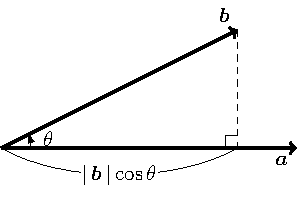
\includegraphics[width=6cm]{picture/vecter1.pdf}
 \caption{内積は何を表すか}
\end{figure}

$\lvert \bm{b} \rvert \cos \theta$というのは
$\bm{b}$が$\bm{a}$の方向にどれだけの長さを持っているかを表しているのである.
もちろん$\lvert \bm{a} \rvert \cos \theta$という部分を考えてもよい.
このとき,この量は$\bm{a}$が$\bm{b}$の方向にどれだけの長さを持っているかを表している.
いまは3次元空間でやってみたが,$n$次元空間でもそうなっていると思ってみよう.
$n$次元空間での角度や方向など意味不明だが,3次元空間でのイメージをそのまま持ってくるのである.
つまり,ベクトルの内積は
片方のベクトルがもう片方のベクトルの方向
にどれだけの長さを持っているかを表しているのである.
この解釈は今後もよく使うので覚えておいていただきたい.

この解釈から,
2つのベクトルが直交するための条件は,
そのベクトルの内積が0になることであるという重要な事実がわかる.
数学的にいえば$\theta = 90^\circ$のとき$\cos \theta = 0$になるということである.

ベクトルの内積に関してはこんなものである.演習を1つしてみようか.
\begin{itembox}[l]{問}
3次元空間において,2つのベクトル$\bm{a}, \, \bm{b}$の内積を,
$\bm{a}$と$\bm{b}$のなす角を$\theta$として
$$
\bm{a} \cdot  \bm{b} = \lvert \bm{a} \rvert \lvert \, \bm{b} \rvert \cos \theta
$$
と\.定\.義したとき,
$$
\bm{a} \cdot \bm{b} = a_1 b_1 +a_2 b_2 + a_3 b_3
$$
が成り立っていることを\.証\.明せよ.ただし
$$
\lvert \bm{a} \rvert = \sqrt{a_1^2 + a_2^2 + a_3^2} \ ,\ \lvert \bm{b} \rvert = \sqrt{b_1^2 + b_2^2 + b_3 ^2}
$$
である.
\end{itembox}
\subsection{単位ベクトルと標準基底}
ベクトルを使っていると,あるベクトルの向きだけを利用したいということがよくある.
たとえば,$\bm{r}$と同じ方向を向いていて,大きさ$\displaystyle \frac{1}{4 \pi \varepsilon_0} \frac{q}{r^2}$
のベクトルを考えたいなどである.こういうことはよくある.そのための手法は割と簡単なので知っておこう.

ベクトル$\bm{r}$の大きさを$r$と書く.これは物理ではよくやる書き方である.この$r$で$\bm{r}$を割ったものを考えれば,
その大きさは1になる.このベクトルは$\displaystyle \frac{\bm{r}}{r}$である.
そして,このベクトルの方向は,もちろん$\bm{r}$と同じ方向を向いている.
このベクトルに大きさである
$\displaystyle \frac{1}{4 \pi \varepsilon_0} \frac{q}{r^2}$をかけてやれば目的のベクトルが得られる.
これを$\bm{E}$と書けば,
$$
\bm{E} = \frac{1}{4 \pi \varepsilon_0} \frac{q}{r^2} \frac{\bm{r}}{r} 
$$
となるのである.\footnote{これは静電場である.}

このように,大きさが1のベクトルは何かと使いやすい.その向きだけを自由に使えるからである.
大きさが1のベクトルを\emph{単位ベクトル}\index[widx]{べくとる@ベクトル!たんい@単位---}
という.
大きさが1だから``単位''である.

さて,単位ベクトルのなかで,次のようなものを考えてみよう.
\begin{align}
\bm{e}_1 = \left[ 
 \begin{array}{c}
  1 \\
  0 \\
  0 \\
  \vdots \\
  0
 \end{array}
 \right]
  , \, 
 \bm{e}_2 = \left[ 
 \begin{array}{c}
  0 \\
  1 \\
  0 \\
  \vdots \\
  0
 \end{array}
 \right]
 \, , \, 
 \cdots 
 , \, 
 \bm{e}_n = \left[ 
 \begin{array}{c}
  0 \\
  0 \\
  0 \\
  \vdots \\
  1
 \end{array}
 \right]
 \label{eq:hyoujunnkitei}
\end{align}
これらはすべて単位ベクトルで,すべてのベクトルが互いに直交している.
この集団$\{ \, \bm{e}_1, \, \bm{e}_2, \, \cdots , \, \bm{e}_n \, \}$を
$n$次元数ベクトル空間の\emph{標準基底}
\index[widx]{きてい@基底!ひょうじゅん@標準---}と呼ぶ.
なぜか$ \{ \cdots \} $がついているが,ベクトルを集めてこれらをまとめて扱うとき,
こういう風にカッコでまとめるのが習わしである.
しかし集合を表すカッコとはまたちょっと違うのだそうだ.
なんだそれ? という感じである.
話を戻そう.$n$次元数ベクトル空間のすべてのベクトルはこれらの標準基底の組み合わせで表すことができる.
実際,任意のベクトル$\bm{a}$を成分表示して
$$
\bm{a} = \left[
 \begin{array}{c}
  a_1 \\
  a_2 \\
  \vdots \\
  a_n
 \end{array}
 \right]
$$
と書き表すとき,$\bm{a}$は
\begin{align}
\bm{a} = a_1 \bm{e}_1 + a_2 \bm{e}_2 + \cdots + a_n \bm{e}_n
\label{eq:veckiteihyougenn}
\end{align}
と書き表すことができる.この形式もよく使うので覚えておいてもらいたい.

また,3次元数ベクトル空間においては,標準基底を$\bm{e}_x, \, \bm{e}_y, \, \bm{e}_z$と表したり,
$\bm{i} , \, \bm{j}, \, \bm{k}$などと表したりすることがある.
力学なんかだとよく$\bm{i}, \, \bm{j}, \, \bm{k}$という表現を目にすることがあるだろう.
その本において記号がどういう意味で使われているのかはまちまちであるから,逐一確かめる癖をつけておこう.

ともかく,これで外積をやる準備が整った.とっとと片づけてしまおう.
\subsection{ベクトルの外積}
ベクトルの積は2種類あるといった.1つはさっきやった内積である.もう1つはこれからやる外積である.
内積はベクトル2つから1つの実数を作り出す演算であったが,外積はベクトル2つから新たなベクトルを1つ作り出す演算である.

また,内積は一般の$n$次元の数ベクトル空間で定義したが,外積に関しては3次元空間に限らせてもらう.
外積を一般の$n$次元の数ベクトル空間に拡張できないこともないのだが,
内積と違って話がかなり複雑になってしまうことが知られている.\footnote{超複素数なる理論を使うらしい.}
そんなことをしても物理学を学ぶ上であまりいいこともないので,とりあえず3次元空間で話をしよう.
\subsubsection{まずは定義から}
外積の定義は,内積のときと同じく幾何学的に定義する手法と成分表示で定義する手法との2種類あるのだが,
今回は幾何学的に定義する方でやってみよう.

2つのベクトル$\bm{a}, \, \bm{b}$について,その外積を$\bm{a} \times \bm{b}$と書く.
\index[widx]{べくとる@ベクトル!のがいせき@---の外積}
``$\times$''は``クロス''と読むのが一般的らしい.``$\bm{a} \times \bm{b}$''は``$\bm{a}$クロス$\bm{b}$''と読むのである.
このことから,ベクトルの外積は\emph{クロス積}
\index[widx]{べくとる@ベクトル!のくろすせき@---のクロス積}とも呼ばれる.
ただ,``$\times$''を普通に``かける''と呼んでしまう人も多い.


外積はベクトルである.ベクトルというからには向きと大きさがあるはずだ.
逆に,向きと大きさが決まればベクトルはただ1つに定まるといえる.
そこで,ベクトルの外積をその向きと大きさにわけて定義しよう.

外積$\bm{a} \times \bm{b}$の大きさは,$\bm{a}$と$\bm{b}$がなす角を$\theta$として
\begin{align}
\lvert \bm{a} \times \bm{b} \rvert = \lvert \bm{a} \rvert \lvert \bm{b} \rvert \sin \theta 
\label{eq:gaisekiookisa}
\end{align}
であると定義する.これは,$\bm{a}$と$\bm{b}$が張る平行四辺形の面積を表している.
\begin{figure}[h]
 \centering
 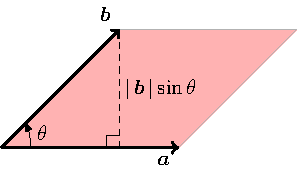
\includegraphics[width=5.5cm]{picture/vecter2.pdf}
 \caption{2つのベクトルが張る平行四辺形}
\end{figure}

図に赤色で示した領域が$\bm{a}$と$\bm{b}$が張る平行四辺形であり,
$\lvert \bm{a} \rvert$がその底辺,$\lvert \bm{b} \rvert \sin \theta$がその高さになっている.
内積のときは$\cos$を使ったのに対して外積の大きさは$\sin$である.
外積の大きさは2つのベクトルが直交している状態に近いほど大きくなるのである.
対して内積の値は2つのベクトルが平行である状態に近いほど値は大きくなり,直交しているときにはその値は0になるのだった.
結果がベクトルかスカラーかの違いはあるものの,内積と外積はなかなか対称的なものになっている.

次は向きである.外積$\bm{a} \times \bm{b}$の向きは$\bm{a}$から$\bm{b}$の向きに右ネジを回したとき,
そのネジが進む方向であると定義する.
\begin{figure}[h]
 \centering
 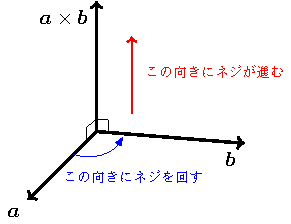
\includegraphics[width=6cm]{picture/vecter3.pdf}
 \caption{外積の向き}
\end{figure}

2つのベクトル$\bm{a}, \, \bm{b}$とその外積$\bm{a} \times \bm{b}$の向きの関係はこのようになっている.
``右ネジ''という言葉になじみがなければ自分の右手を見てほしい.親指以外の指をガッツポーズを緩めた感じに丸めてみる.
一種の渦のようなものが見えただろうか.指の根元から先に向かって渦が巻いているイメージである.
そして,そのときに親指が向いている方向がネジの進む方向になっている.``右手''だから``右ネジ''なのである.
親指以外の指をガッツポーズを緩めた感じに丸め,$\bm{a}$の方向を指の根元に,そして$\bm{b}$の方向に指の先を向けてほしい.
そして,そのとき親指が指し示す方向が外積$\bm{a} \times \bm{b}$の方向である.右ネジよりもこちらの方が覚えやすいかもしれない.
なによりいつでも再現できる.私は右ネジの覚え方より右手の覚え方の方が好きである.読者の方々はどうだろうか? 

ネジの回転面とネジの進む方向は明らかに直交している.つまり,
\begin{align}
\bm{a} \cdot ( \, \bm{a} \times \bm{b} \, ) = 0 \: , \:  \bm{b} \cdot ( \, \bm{a} \times \bm{b} \, ) =0 
\label{eq:naisekigaiseki}
\end{align}
という関係式が成り立っている.右辺の0はスカラー量である.
式中にあるカッコは重要である.左側では$\bm{a}$というベクトルと$\bm{a} \times \bm{b}$というベクトルの内積をとっている.
これを
\begin{align*}
\bm{a} \cdot \bm{a} \times \bm{b}
\end{align*}
のように書いてしまうようなことはしてはいけない.カッコはモノのかたまりを表すのである.
また,式(\ref{eq:naisekigaiseki})が成り立っていることは図を見てもらえれば納得できるはずだ.
直交する2つのベクトルの内積は0になるのだった.

そういえば,上の説明で$\bm{a} \times \bm{b}$と$\bm{b} \times \bm{a}$が異なったベクトルになるということはわかるだろうか? 
ネジを回す向きを逆にすればネジが進む方向も逆になる.
$\bm{a} \times \bm{b}$と$\bm{b} \times \bm{a}$とで向きは逆になる.しかし大きさは変わらないだろう.
つまり,次のような等式が成り立っているということである.
\begin{align}
\bm{a} \times \bm{b} = - ( \, \bm{b} \times \bm{a} \, ) 
\label{eq:gaisekihantaisyou}
\end{align}
対して,ベクトルの内積は順序を逆にしても結果は変わらない.
\begin{align}
\bm{a} \cdot \bm{b} = \bm{b} \cdot \bm{a}
\label{eq:naisekitaisyou}
\end{align}
意味を考えれば明らかである.特に悩むようなこともないだろう.

\subsubsection{外積の成分表示}
さて,外積の向きと大きさを定義したので外積がきっちり定義できたことになる.
しかし,これでは外積を具体的に計算することは困難である.
やっぱり成分表示してある方がなにかと便利である.それを求めてみよう.

\subsubsection{まずは簡単な場合から}
まずは$\bm{a}$と$\bm{b}$が$xy$平面上のベクトルである場合を考えよう.
$$
\bm{a} = \left[
 \begin{array}{c}
  a_x \\ 
  a_y \\
  0
 \end{array}
\right]
\; , \; 
\bm{b} = \left[
 \begin{array}{c}
  b_x \\ 
  b_y \\
  0
 \end{array}
\right]
$$
としてみる.添え字を1や2でなく$x$と$y$を使っているのはこれが$xyz$空間における座標と対応していることを思い出してほしいからである.
さて,外積$\bm{a} \times \bm{b}$は$\bm{a}$と直交し,かつ$\bm{b}$とも直交しているのだった.
したがって,$\bm{a} \times \bm{b}$は$z$軸方向を向いたベクトルであるはずで,
$\bm{a} \times \bm{b}$の$x$成分と$y$成分はともに0であるはずだ.
$$
\bm{a} \times \bm{b} = \left[
 \begin{array}{c}
  0 \\
  0 \\
  z
 \end{array}
\right]
$$
という形に書けるはずである.そして,ここから
$$
\lvert \bm{a} \times \bm{b} \rvert = \lvert z \rvert
$$
であることがわかる.
\footnote{実数$z$について,$\sqrt{z^2}=\lvert z \rvert$が成り立つのだった.}
さて,$\lvert \bm{a} \times \bm{b} \rvert$は
$\bm{a}$と$\bm{b}$が貼る平行四辺形の面積を表しているのだった.
そして,この値は
$$
\lvert a_x b_y - a_y b_x \rvert
$$
である. これは各自確かめてほしい.このことから
$$
\lvert z \rvert = \lvert a_x b_y - a_y b_x \rvert
$$
となることがわかり,
$$
z = a_x b_y - a_y b_x \; \text{か,} \; z = - ( a_x b_y - a_y b_x )
$$
のどちらかが成り立っていることになる.いったいどちらだろうか? 結論から言うと
$$
z = a_ x b_y - a_y b_x
$$
が成り立っている.なぜだろうか? これは外積の向きに起因するものである.

思い切り単純な例で考えてみよう.
$$
\bm{a} = \left[
 \begin{array}{c}
  1 \\ 
  0 \\
  0
 \end{array}
\right]
\; , \; 
\bm{b} = \left[
 \begin{array}{c}
  0 \\ 
  1 \\
  0
 \end{array}
\right]
$$
としてみると,
$$
\bm{a} \times \bm{b} = \left[
 \begin{array}{c}
  0 \\
  0 \\
  1
 \end{array}
\right]
$$
となる.各自図を描くなり右手を使うなりして確かめてほしい.この例を考えれば
$$
z = a_x b_y - a_y b_x
$$
となっていることも納得がいくはずである.すなわち
$$
\bm{a} \times \bm{b} = \left[
 \begin{array}{c}
  0 \\
  0 \\
  a_x b_y - a_y b_x
 \end{array}
\right]
$$
となるわけだ.

これとまったく同様にして,$yz$平面上の2つのベクトル
$$
\bm{a} = \left[
 \begin{array}{c}
  0 \\ 
  a_y \\
  a_z
 \end{array}
\right]
\; ,\; 
\bm{b} = \left[
 \begin{array}{c}
  0 \\ 
  b_y \\
  b_z
 \end{array}
\right]
$$
に対しては
$$
\bm{a} \times \bm{b} = \left[
 \begin{array}{c}
  a_y b_z - a_z b_y \\
  0 \\
  0
 \end{array}
\right]
$$
となるし,$zx$平面上の2つのベクトル
$$
\bm{a} = \left[
 \begin{array}{c}
  a_x \\ 
  0 \\
  a_z
 \end{array}
\right]
\; , \; 
\bm{b} = \left[
 \begin{array}{c}
  b_x \\ 
  0 \\
  b_z
 \end{array}
\right]
$$
に対しては
$$
\bm{a} \times \bm{b} = \left[
 \begin{array}{c}
  0 \\
  a_z b_x - a_x b_z \\
  0
 \end{array}
\right]
$$
となっていることがわかる.これも各自確かめてほしい.

以上の考察から,一般の$xyz$空間の2つのベクトル
$$
\bm{a} = \left[
 \begin{array}{c}
  a_x \\ 
  a_y \\
  a_z
 \end{array}
\right]
\; , \; 
\bm{b} = \left[
 \begin{array}{c}
  b_x \\ 
  b_y \\
  b_z
 \end{array}
\right]
$$
に対しては
\begin{align}
\bm{a} \times \bm{b} = \left[
 \begin{array}{c}
a_y b_z - a_z b_y \\
a_z b_x - a_x b_z \\
a_x b_y - a_y b_x
\end{array}
\right]
\label{eq:gaisekiseibun}
\end{align}
となっていると推測できる.実際これは成り立っているのだが,詳しく話すとやや面倒になるので割愛させてもらう.

\subsubsection{外積の成分表示の覚え方}
外積の成分表示はやや複雑な式で覚えにくい.だが,毎回成分表示の公式を導くのはさすがに面倒である.
添え字の並びに何か規則性を見出せそうだ.

まずは$x$成分の$a_y b_z - a_z b_y$を見てみよう.$x$成分には添え字に$x$が表れていない.そして,
前半の$a_y b_z$と後半の$a_z b_y$はちょうど添え字が入れ替わった形になっている.

次は$y$成分の$a_z b_x - a_x b_z$という部分について考えてみる.これも$y$成分には添え字に$y$が出てこないし,
$a_z b_x$と$a_x b_z$はちょうど添え字が入れ替わった形になっている.

$z$成分に関しても同様である.いちいち書かなくてもいいだろう.``添え字を入れ替えて引く''という規則性がありそうだ.
図式化してみよう.例えばこんな感じである.
\begin{figure}[h]
 \centering
 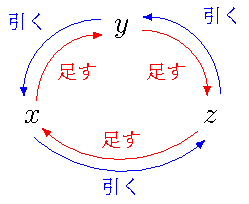
\includegraphics[width=5cm]{picture/vecter4.pdf}
 \caption{外積の成分表示の覚え方}
\end{figure}

$\bm{a} \times \bm{b}$を求めたいときは,
成分を$\bm{a}$のもの,$\bm{b}$のもの,$\bm{a}$のもの,$\bm{b}$のもの,$\cdots$と取り出していく.
図に書いたのは添え字のパターンである.

まず$x$成分からスタートである.一番上の$y$からスタートする.そして右下の$z$に移る.$y, \, z$という添え字の配列が与えられる.
こうして$a_y b_z$というものが与えられる.次に添え字を入れ替えて引くのだ.$a_y b_z - a_z b_y$となる.
これは外積$\bm{a} \times \bm{b}$の$x$成分であった.

次に$y$成分である.さっき進んだ$z$からスタートだ.添え字の配列は$x$に向かって$z, \, x$とする.
そして$a_z b_x$のいうものが得られた.
そして添え字を入れ替えて引くのだ.$a_z b_x - a_x b_z$となり,これは外積$\bm{a} \times \bm{b}$の$y$成分であった.

$z$成分も同様である.外積$\bm{a} \times \bm{b}$の$z$成分は$a_x b_y - a_y b_x$であった.

小難しく図の読み方を書いたが,図を見てどう読むかが直感的にわかったのならそれでいい.とにかく覚えられればいいのだ.

外積に関してはこんなものである.特に難しいところはなかった.わかってしまえばなんてことはないのである.
\begin{itembox}[l]{課題}
3次元数ベクトル空間における標準基底
$$
\bm{e}_x = \left[
 \begin{array}{c}
 1 \\
 0 \\
 0 
 \end{array}
\right]
\: ,\: 
\bm{e}_y = \left[
 \begin{array}{c}
 0 \\
 1 \\
 0 
 \end{array}
\right]
\: ,\: 
\bm{e}_z = \left[
 \begin{array}{c}
 0 \\
 0 \\
 1 
 \end{array}
\right]
$$
について,それらの外積を考える.このとき
$$
\bm{e}_x \times \bm{e}_y = \bm{e}_z \; , \; 
\bm{e}_y \times \bm{e}_z = \bm{e}_x \; , \; 
\bm{e}_z \times \bm{e}_x = \bm{e}_y 
$$
が成り立っていることを
\begin{enumerate}
\item 幾何学的定義に基づいて向きと大きさを求める
\item 成分表示の公式により外積の各成分を直接計算する 
\end{enumerate}
この2つの方法によって確かめよ.

また,2つのベクトル
$$
\bm{a} = \left[
 \begin{array}{c}
  a_x \\ 
  a_y \\
  a_z
 \end{array}
\right]
\; , \; 
\bm{b} = \left[
 \begin{array}{c}
  b_x \\ 
  b_y \\
  b_z
 \end{array}
\right]
$$
と上に述べた標準基底に対して,等式
\begin{align}
\bm{a} \times \bm{b} = \left| 
\begin{array}{ccc}
 \bm{e}_x & \bm{e}_y & \bm{e}_z \\
 a_x & a_y & a_z \\
 b_x & b_y & b_z 
\end{array}
\right|
\label{eq:gaisekidet}
\end{align}
が成り立っていることを確かめよ.ただし右辺の$\lvert \, \cdot \, \rvert$
は行列式を表す.

さらに,3つのベクトル$\bm{a}, \, \bm{b}, \, \bm{c}$について,結合律
\begin{align}
( \bm{a} \times \bm{b} ) \times \bm{c} =\bm{a} \times ( \bm{b} \times \bm{c} )
\end{align}
が成り立っているかどうか検証せよ.

結合律のついでに,交換律や分配律が
内積や外積においてはどうなっているか調査せよ.
\end{itembox}
\section{ベクトル空間の基底とその変換}
さっき``標準基底''という言葉が出てきた.
それらは空間内に存在するベクトルをすべて標準基底を用いて表すことができるのであった.
しかし,空間内のベクトルを表現することに標準基底を用いなければいけないわけではない.
このことについて考えたいのだが,先に少し下準備をしておく.
\subsection{ベクトル空間とは何か}
いままで出てきたのは,$n$次元数ベクトル空間というひどく抽象化されたよくわからない空間であった.
$1,\, 2, \, 3$次元くらいならイメージがつくが,それ以上になるともはや頭の中ではイメージ不可能なものであった.
しかし,ここには大きな落とし穴が潜んでいる.実は,$n$次元数ベクトル空間の``空間''と,
我々が常日頃使っている\footnote{一般の日常生活でという意味である.}``空間''はまったく別物なのである.
いや,さすがに言い過ぎである.
正確には,数学者のいう空間は,我々が空間といってイメージする概念をさらに抽象化したものであるというべきだろうか.

集合に,なんらかの数学的構造を付与したものを\emph{空間}という.
そして,集合に和とスカラー倍という数学的構造を付与したものを\emph{ベクトル空間}
\index[widx]{べくとるくうかん@ベクトル空間}
もしくは\emph{線形空間}\index[widx]{せんけいくうかん@線形空間|see{ベクトル空間}}
と呼ぶ.
数学的構造というとなんとなく難しく聞こえるが,誤解を恐れずにいってしまうと,
数学的構造とはなんらかの``仕組み''である.
ベクトルの演算として,和とスカラー倍というのがあった.
あのような演算ができなければベクトル空間とは言わない.
和やスカラー倍という``仕組み''は数学者的には代数的構造に分類されるらしい.
そういえば,ベクトル空間の性質を探るのは線形代数学の役目であり,
線形代数学には代数学という名前がついているのであった.
こうなると,普通の幾何ベクトルだけでなく,
もっとたくさんの集合がベクトル空間として扱えそうである.
モノの中身でなく,モノが示す性質について議論しているがためにこういうことが言える.
線形代数学の理論がいろいろなところで顔を出すのはこのためである.
いろんな分野で扱う概念にベクトル空間と同じような代数構造を持っているがために,
ベクトル空間の理論を使ってそれらの分野の研究ができるのである.
ただし,物理学では,ベクトル空間にさらに内積と呼ばれる代数構造を付与したものを扱うのが普通である.
内積が付与されたベクトル空間は\emph{計量ベクトル空間}
\index[widx]{べくとるくうかん@ベクトル空間!けいりょう@計量---|see{内積空間}}もしくは
\emph{内積空間}\index[widx]{ないせきくうかん@内積空間}と呼ばれる.
詳しいことは省くが,内積という演算を導入することにより,
ベクトルの長さやなす角といった概念を考えることができるのである.
以前述べた内積のところを読み返してみれば,
ベクトルの長さやなす角(の余弦)といった概念に内積が関与していることがわかるはずだ.

これからはただの数ベクトル空間ではなく一般のベクトル空間の話をするが,
ほとんど普通の数ベクトル空間だと思って解釈してもらって構わない.
そういうことができるよううまいこと理論が組まれているのである.
\subsection{線形結合と線形独立}
2つのベクトル$\bm{a}, \, \bm{b}$とスカラー$p, \, q$について,
\begin{align}
p\bm{a}+q\bm{b}
\label{eq:senkeiketugou}
\end{align}
と表されるベクトルを$\bm{a}$と$\bm{b}$の($p, \, q$を係数とする)\emph{線形結合}
\index[widx]{せんけいけつごう@線形結合}
もしくは\emph{$1$次結合}
\index[widx]{いちじけつごう@1次結合|see{線形結合}}という.
形が何となく比例の式に似ている.比例式はグラフにすると直線を表すので``線形''と呼ばれているのである.
本書は線形結合という呼称を用いることにする.
また,$n$本のベクトル$\bm{v}_1, \, \bm{v}_2, \, \cdots, \, \bm{v}_n$
と$n$個のスカラー$c_1, \, c_2, \, \cdots, \, c_n$について,
\begin{align}
c_1 \bm{v}_1 + c_2 \bm{v}_2 + \cdots + c_n \bm{v}_n
\label{eq:nsenkeiketugou}
\end{align}
と書き表されるベクトルを$\bm{v}_1, \, \bm{v}_2, \, \cdots , \, \bm{v}_n$の
($c_1, \, c_2, \, \cdots, \, c_n$を係数とする)\emph{線形結合}という.
線形結合は,線形代数学の理論の中核をなす非常に重要な概念である.
よく``このベクトルを別のベクトルで表す''ということがあるが(本書でもすでに散々使っている),
これは線形結合で表せるという意味で使うことがほとんどである.
例えば,3次元数ベクトル空間の標準基底$ \{ \, \bm{e}_1, \, \bm{e}_2, \, \bm{e}_3 \, \} $を考えてみる.
ベクトルの外積を用いると,$\bm{e}_3$は$\bm{e}_3 = \bm{e}_1 \times \bm{e}_2$と表せる.
しかし,このような場合,``$\bm{e}_3$は$\bm{e}_1$と$\bm{e}_2$で表せる''とは普通は言わない.
線形結合以外の方法を使っているからである.
$\bm{e}_3$は$\bm{e}_1$と$\bm{e}_2$では表せない.それだけではなく,
$\{ \, \bm{e}_1, \, \bm{e}_2, \, \bm{e}_3 \, \}$からどのベクトルを取り出してきても,
そのベクトルを残った2つのベクトルを用いては表せない.
これを確かめるのは簡単であるから,読者の方々の練習問題としよう.

さて,この``線形結合では表せない''ということについてもう少し考えてみよう.
2つのベクトル$\bm{v}_1, \, \bm{v}_2$について,$\bm{v}_2$が$\bm{v}_1$の線形結合で表せるというのは,
スカラー$c$をうまくとって,$\bm{v}_2 = c \bm{v}_1$が成り立つということである.
式(\ref{eq:nsenkeiketugou})はベクトルが複数あるが,いまは1つのベクトルだけで線形結合というものを考えている.
この場合は$c \bm{v}_1$というただのスカラー倍に相当するわけだ.
ベクトルのスカラー倍というのはベクトルが表現する矢印を伸ばしたり縮めたりするようなイメージであった.
従って,$\bm{v}_2$が$\bm{v}_1$の線形結合で表せるというのは,$\bm{v}_1$と$\bm{v}_2$の向きが同じであるか,
違ったとしても向きが真逆であるかのどちらかである.
この場合,``$\bm{v}_1$と$\bm{v}_2$を用いて別のベクトルを表現する''という観点では
2本もベクトルはいらないということに
なる.\footnote{この``表現する''ももちろん線形結合で表現するという意味である.}
このとき,$\bm{v}_1$と$\bm{v}_2$の線形結合全体の集合は,ある種の直線のような集合になる.
よって,この集合は1次元のベクトル空間であるといわれるのだ.
次元についてはあとで詳しくやろう.

次に,$\bm{v}_2$が$\bm{v}_1$の線形結合で表せないとしよう.
この場合,$\bm{v}_1$と$\bm{v}_2$の向きはまったく違うことになる.違うといっても正反対ではあってはならない.
``$\bm{v}_1$と$\bm{v}_2$を用いて別のベクトルを表現する''という観点で考えてみると,
この2つのベクトルは$\bm{v}_1$と$\bm{v}_2$の貼る
平面\footnote{内積のところで``2つのベクトルが貼る平行四辺形''というのをやったが,それと同じイメージである.}
内に存在するベクトルすべてを表すことができる.
しかし,ひとたびその平面から飛び出てしまったベクトルは,$\bm{v}_1$と$\bm{v}_2$では表せない.
平面を表すので,このベクトル空間は2次元であるといわれるのである.
また,$\bm{v}_1$と$\bm{v}_2$が貼る平面から飛び出すようなベクトル$\bm{v}_3$をとり,
$\bm{v}_1, \, \bm{v}_2, \, \bm{v}_3$の3本のベクトルの線形結合全体からなる集合を考えると,
この集合は空間上のあらゆる点全部の集合である.
というわけで,このベクトル空間は3次元であるといわれる.

\subsection{ベクトル空間の基底と次元}
ここまでもったいぶって引っ張ってきた線形独立性について話をしよう.
\begin{itembox}[l]{定義}
$n$本のベクトル$ \bm{v}_1, \, \bm{v}_2, \, \cdots, \, \bm{v}_n $について,
\begin{align}
c_1 \bm{v}_1 + c_2 \bm{v}_2 + \cdots + c_n \bm{v}_n = 0
\label{eq:senkeidokuritu}
\end{align}
を成り立たせるスカラー$c_1, \, c_2, \, \cdots , \, c_n$が$c_1=c_2=\cdots=c_n=0$以外にないとき,
$ \bm{v}_1, \, \bm{v}_2, \, \cdots, \, \bm{v}_n $は
\emph{線形独立}\index[widx]{せんけいどくりつ@線形独立}
であるといい,式(\ref{eq:senkeidokuritu})を成り立たせる
スカラー$c_1, \, c_2, \, \cdots , \, c_n$が$c_1=c_2=\cdots=c_n=0$以外に存在するとき,
$ \bm{v}_1, \, \bm{v}_2, \, \cdots, \, \bm{v}_n $は
\emph{線形従属}\index[widx]{せんけいじゅうぞく@線形従属}であるという.
\end{itembox}
線形独立と線形従属はそれぞれ1次独立,1次従属とも呼ばれる.これは線形結合と同じである.
さっきまでの話とずいぶん趣が違うように見えるがそれは表現上の都合である.
それを象徴するような定理がある.
\begin{itembox}[l]{定理}
$n$本のベクトル$ \bm{v}_1, \, \bm{v}_2, \, \cdots, \, \bm{v}_n $について,
$ \bm{v}_1, \, \bm{v}_2, \, \cdots, \, \bm{v}_n $が線形独立であるための必要十分条件は,
$ \bm{v}_1, \, \bm{v}_2, \, \cdots, \, \bm{v}_n $の中からどのベクトルをとっても,
そのベクトルが残ったベクトルの線形結合で書き表せないことである.
\end{itembox}
この定理の証明もあまり難しくないので読者への課題としておこう.
線形独立のイメージとしては今述べた定理のようなイメージであるが,
数学の議論を進めていくうえで使いやすいのは定義で述べた方である.
しかし,どちらも同じことだよというのが数学の議論によって証明できるので,
どちらを定義として採用しても構わない.
実際,定理として述べた上の命題を定義として採用している本も多い.
また,これまでの議論から,次元と線形独立性が非常に深く関係していることが見て取れる.

さて,我々は``次元''という言葉をあいまいに使ってきた.そこで,次元という言葉を正確に定義しておこう.
\begin{itembox}[l]{定義}
ベクトル空間$V$と,$V$の$n$本のベクトル$ \bm{v}_1, \, \bm{v}_2, \, \cdots, \, \bm{v}_n $について,
$ \bm{v}_1, \, \bm{v}_2, \, \cdots, \, \bm{v}_n $が線形独立で,かつ
$V$のどんなベクトルも$ \bm{v}_1, \, \bm{v}_2, \, \cdots, \, \bm{v}_n $の線形結合で表せるとき,
$ \bm{v}_1, \, \bm{v}_2, \, \cdots, \, \bm{v}_n $は$V$の\emph{基底}
\index[widx]{きてい@基底}
である,もしくは単に\emph{基}といい,$V$は\emph{$n$次元}ベクトル空間であるという.
\end{itembox}
我々がいままでなんとなく使ってきた``次元''という言葉は,
ベクトル空間のなかのベクトルを表現するのに必要な最低限のベクトルの本数だということになる.
\footnote{しかし,我々はもうひとつ別の``次元''という言葉の使い方を知っている.}
``必要''が$V$のどんなベクトルもの部分に対応し,``最低限''が線形独立性に対応している.
上に書いた無機質で数学チックな``次元''の定義がいままで何も考えずに使っていた``次元''という言葉の
ニュアンスとぴったり合致していることはわかるだろうか? 我々が生きているこの世界が
ベクトル空間であるかどうかに関しては疑問の余地は大いにあるが,
そういう細かいことを無視すれば,``次元''という言葉のイメージと厳密な定義がぴったり一致したはずである.
なお,先ほど述べた定義は暗に次元が有限であることを前提にしている.
有限個の基底をとることができないような無限次元のベクトル空間も確かに存在してはいるのだが,
そういう話をしだすとめんどくさいのでここでは述べない.
近いうちに出会うことになるだろうからそのときに学んでもらえばいい.

もうひとつ重要な話をしなければならない.
それは,ベクトル空間が与えられたとき,
その基底の取り方は何通りも考えられるということである.
これは結構重要な事実である.
例を出して考えよう.3次元数ベクトル空間$\mathbb{R}^3$において,
\footnote{数ベクトル空間を表すときはこういう変な文字を使う.
手書きではベクトルと同じように2重文字で書いておけばよい.}
標準基底
\begin{align*}
\bm{e}_1 = \left[
 \begin{array}{c}
  1 \\ 
  0 \\
  0
 \end{array}
\right]
\; , \, \; 
\bm{e}_2 = \left[
 \begin{array}{c}
  0 \\ 
  1 \\
  0
 \end{array}
\right]
\; , \; 
\bm{e}_3 = \left[
 \begin{array}{c}
 0 \\
 0 \\
 1
 \end{array}
\right]
\end{align*}
はもちろん$\mathbb{R}^3$の基底である.だが,
\begin{align*}
\bm{a}_1 = \left[
 \begin{array}{c}
  1 \\ 
  1 \\
  0
 \end{array}
\right]
\; , \, \; 
\bm{a}_2 = \left[
 \begin{array}{c}
  0 \\ 
  1 \\
  1
 \end{array}
\right]
\; , \; 
\bm{a}_3 = \left[
 \begin{array}{c}
 1 \\
 0 \\
 1
 \end{array}
\right]
\end{align*}
としてみるとこれら$ \{ \, \bm{a}_1, \, \bm{a}_2, \, \bm{a}_3 \, \} $も$\mathbb{R}^3$の基底になっている.
本当に基底になっているかどうか確かめる作業は読者にゆだねよう.そんなに難しい話ではない.
基底の取り方はいろいろあるが,
同じベクトル空間であるならば基底の数は取り方によらず一定であることが知られている.
あるベクトル空間$V$において,とある基底をとってみたら4本だったが,
別の取り方をしてみたら3本でしたということはあり得ない.
ベクトル空間の次元は基底の取り方には依存しないのである.
もし依存するようなことがあれば,ベクトル空間の次元は基底ごとに変化するということになってしまう.
このようなことは直感的に考えてもあり得なさそうだということはわかるだろう.
この事実は数学的に証明できるものであるが本書ではスキップしておく.

さらに1つ補足をしておく.$n$次元ベクトル空間$V$の基底を1つとり,
$V$のベクトルをその基底の線形結合として表したとき,その表し方は一意である.
これは直感的にも納得できるだろう.もちろん数学的にも簡単に証明できる.

そういえば,$ \{ \, \bm{e}_1, \, \bm{e}_2, \, \bm{e}_3 \, \} $は$\mathbb{R}^3$の基底であって,
$ \{ \, \bm{a}_1, \, \bm{a}_2, \, \bm{a}_3 \, \} $も同じ$\mathbb{R}^3$の基底であった.
従って,互いは互いの線形結合で表せるはずである.
実際,
\begin{align*}
\bm{a}_1 = 1 \bm{e}_1 + 1 \bm{e}_2 + 0 \bm{e}_3 \\
\bm{a}_2 = 0 \bm{e}_1 + 1 \bm{e}_2 + 1 \bm{e}_3 \\
\bm{a}_3 = 1 \bm{e}_1 + 0 \bm{e}_2 + 1 \bm{e}_3 
\end{align*}
となる.ここで,行列$A$を
\begin{align*}
A= \left[
\begin{array}{ccc}
1 & 0 & 1 \\
1 & 1 & 0 \\
0 & 1 & 1
\end{array}
\right] 
\end{align*}
と定めてみると,
\begin{align}
\left[
\begin{array}{ccc}
\bm{a}_1 & \bm{a}_2 & \bm{a}_3 
\end{array}
\right]
= 
\left[
\begin{array}{ccc}
\bm{e}_1 & \bm{e}_2 & \bm{e}_3
\end{array}
\right]
A
\label{eq:ahenkan}
\end{align}
という関係式が成り立つ.
この式は,行列の積のルールにのっとった関係式
\begin{align*}
\left[
\begin{array}{ccc}
1 & 0 & 1 \\
1 & 1 & 0 \\
0 & 1 & 1 
\end{array}
\right]
= 
\left[
\begin{array}{ccc}
1 & 0 & 0 \\
0 & 1 & 0 \\
0 & 0 & 1 \\
\end{array}
\right]
\left[
\begin{array}{ccc}
1 & 0 & 1 \\
1 & 1 & 0 \\
0 & 1 & 1
\end{array}
\right]
\end{align*}
というところからきている.
それぞれのベクトルや行列の成分を代入してみればすぐにわかるはずだ.
行列$A$の定義が列と行が逆に見えたのは,各列ベクトルを横に配置しているからである.
関係式を並べるときには各ベクトルを縦に並べ,さも1つの未知数であるかのように表した.
連立方程式を行列で表記したのと同じように見せるためだ.
しかし,いま扱っているモノは未知数ではなくベクトルである.
そういう場合には違う表記をした方が都合がいい.
まぁどう都合がいいかを説明しろと言われると困るのだが.
ともかく,この関係式はこの後すぐに使うので頭の片隅にでも置いておいてほしい.
\subsection{基底の変換}
ここまで長々とおおよそ物理と関係のなさそうなことを述べてきたのはもちろんわけがある.
抽象的な数学が何を目指しているかを知ってほしいというのも1つであるが,
最大の目的は基底の変換という概念をマスターすることにある.
さっき述べた話とつながるのだが,復習を兼ねてもう一度最初から説明してみよう.
ただし,もはや扱うのは数ベクトルではなく一般のベクトルだ.

あるベクトル空間$V$があったとする.$\bm{v}_1, \, \bm{v}_2, \, \cdots , \, \bm{v}_n$を$V$の基底として取ろう.
しかし,基底の取り方は1通りではない.取り方はいくらでも考えられるのであった.
例えばそれを$\bm{v}'_1, \, \bm{v}'_2, \, \cdots , \, \bm{v}'_n$としてみよう.
基底の取り方はいろいろあるが,その本数は変わらないのだった.
というわけでさっきと同じく$n$本である.
さて,$\bm{v}_1, \, \bm{v}_2, \, \cdots , \, \bm{v}_n$と$\bm{v}'_1, \, \bm{v}'_2, \, \cdots , \, \bm{v}'_n$
は,同じベクトル空間$V$の基底である.
従って,互いは互いの線形結合で表せるはずである.
つまり,$n^2$個のスカラー
$p_{11}, \, p_{12}, \, \cdots, \, p_{1n}, \, p_{21}, \, p_{22}, \, \cdots, \, p_{2n}, \, \cdots, \,  p_{nn}$
をうまく選んで
\begin{align}
\begin{aligned}
\bm{v}'_1 & = p_{11} \bm{v}_1 + p_{21} \bm{v}_2 + \cdots + p_{n1} \bm{v}_n \\
\bm{v}'_2 & = p_{12} \bm{v}_1 + p_{22} \bm{v}_2 + \cdots + p_{n2} \bm{v}_n \\
& \hspace{2.3cm }\vdots \\
\bm{v}'_n & = p_{1n} \bm{v}_1 + p_{2n} \bm{v}_2 + \cdots + p_{nn} \bm{v}_n 
\end{aligned}
\label{eq:nanka}
\end{align}
という$n$個の関係式を成立させることができるはずである.
なんだかどこかで見た形である.そこで,$n$次の正方行列$P$を
\begin{align*}
P =
\left[
\begin{array}{cccc}
p_{11} & p_{12} & \ldots & p_{1n} \\
p_{21} & p_{22} & \ldots & p_{2n} \\
\vdots & \vdots & \ddots & \vdots \\
p_{n1} & p_{n2} & \ldots & p_{nn}
\end{array}
\right]
\end{align*}
と定めてみる.
すると,式(\ref{eq:nanka})は次のように変形できる.
\begin{align}
( \bm{v}'_1, \, \bm{v}'_2, \, \cdots, \bm{v}'_n ) = ( \bm{v}_1, \, \bm{v}_2, \, \cdots, \bm{v}_n ) P
\label{eq:henkan}
\end{align}
この話は以前にもやった話である.以前の話と違うのは,ベクトルが$n$本あるということと,
扱っているのが数ベクトルではなく一般のベクトルだということである.
そういうわけで,ベクトルをまとめるカッコが$[ \cdots ]$ではなく$( \cdots )$になっている.
このカッコはとりあえず行列を表すカッコと同じように解釈してくれて構わない.
式(\ref{eq:henkan})は以前やった式(\ref{eq:ahenkan})とほとんど同じことを表しているというわけだ.

さて,ここからが話の核心である.式(\ref{eq:henkan})を作ったときは
``すでに基底が2組与えられていて,それらを行列が結びつけている''というイメージであった.
しかし,こう解釈できないだろうか? すでに基底
$ \{ \bm{v}_1, \, \bm{v}_2, \, \cdots, \, \bm{v}_n \} $と行列$P$が与えられていて,
それを用いて新しい基底$ \{ \bm{v}'_1, \, \bm{v}'_2, \, \cdots, \, \bm{v}'_n \} $を作り出した
のだと解釈してみるのである.
このように考えてみると,行列$P$は基底$ \{ \bm{v}_1, \, \bm{v}_2, \, \cdots, \, \bm{v}_n \} $
を別の基底$ \{ \bm{v}'_1, \, \bm{v}'_2, \, \cdots, \, \bm{v}'_n \} $
に変換するような行列であるとイメージできる.
というわけで,この行列$P$を基底$ \{ \bm{v}_1, \, \bm{v}_2, \, \cdots, \, \bm{v}_n \} $
から基底$ \{ \bm{v}'_1, \, \bm{v}'_2, \, \cdots, \, \bm{v}'_n \} $への\emph{変換行列}
\index[widx]{きてい@基底!のへんかんぎょうれつ@---の変換行列}と名付けよう.
この基底の変換は,そのまま座標変換の話につながってくる.
基底と座標は深くつながっているのである.このことについて考えてみよう.
\section{座標系とその変換}\label{zahyoukei}
\label{sec:zahyoukei}
$n$次元のベクトル空間$V$において,その基底を1つとり,$ \{ \bm{v}_1, \, \bm{v}_2, \, \cdots, \, \bm{v}_n \} $
すると,$V$内の任意のベクトル$\bm{a}$はこれらの基底の線形結合で表せる.
その線形結合を
\begin{align}
\bm{a} = a_1 \bm{v}_1 + a_2 \bm{v}_2 + \cdots + a_n \bm{v}_n 
\label{eq:ketugou}
\end{align}
としてみる.式(\ref{eq:ketugou})中の係数の組$(a_1, \, a_2, \, \cdots , \, a_n)$を
$\bm{a}$の基底$ \{ \bm{v}_1, \, \bm{v}_2, \, \cdots, \, \bm{v}_n \} $に関する
\emph{座標}\index[widx]{ざひょう@座標}
と呼ぶ.
ここに使われている``座標''という言葉は,$n$次元数ベクトル空間$\mathbb{R}^n$において,
我々がこれまで使っていた``座標''とほとんどまったく同じ意味である.
基底として,標準基底$ \{ \, \bm{e}_1, \, \bm{e}_2, \, \cdots , \, \bm{e}_n \, \} $をとれば,
ベクトル$\bm{a} = \left[
\begin{array}{c}
a_1 \\
a_2 \\
\vdots \\
a_n
\end{array}
\right]
$は
\begin{align*}
\bm{a} = a_1 \bm{e}_1 + a_2 \bm{e}_2 + \cdots + a_n \bm{e}_n
\end{align*}
と表されるので,$\bm{a}$の標準基底$ \{ \bm{e}_1, \, \bm{e}_2 , \, \cdots , \, \bm{e}_n \} $に関する座標は
$( a_1, \, a_2, \, \cdots , \, a_n)$ということになる.数ベクトル空間の概念を導入したときと同じようなイメージである.
あのときは$\mathbb{R}^n$の基底を標準基底とするということが暗黙のうちに了解されていたのである.

さて,ここからが面白いところである.同じベクトル空間であっても,その基底の取り方はいろいろあったのだった.
同じベクトルであっても,選ぶ基底が変わればその基底に関する座標は変化する.
つまり,基底を選択することは,その空間でどのような座標系を導入するかに相当するのである.
ここでは,物理でよく使う2次元と3次元数ベクトル空間$\mathbb{R}^2, \, \mathbb{R}^3$
のいろいろな座標系について考えてみよう.
\subsection{2次元空間における座標系}
空間内の座標を決定するためのシステムのことを\emph{座標系}\index[widx]{ざひょうけい@座標系}
と呼ぶ.
座標系は,ほとんど基底と同じようなイメージである.
そして,ある座標系から別の座標系に乗り換えることを\emph{座標変換}
\index[widx]{ざひょう@座標!へんかん@---変換}と呼ぶ.
今回主題になるのは,座標系にはどういうものがあって,それぞれがどういう関係で結びついているかということである.
物理でよく使う座標系にはいくつか種類がある.
寄り道をしながらひとつひとつゆっくり見ていこう.
\subsubsection{直交直線座標系}
まずは2次元空間における座標系について考えよう.2次元に対して``空間''という言い方はあまりしなくて,
普通2次元平面というように呼ばれるのであった.
そういえば,我々はよくこの平面のことを\emph{$xy$平面}というように呼ぶのだった.
なぜかというと,我々は通常右向きに$x$軸,上向きに$y$軸を置き,
それに従って平面上の点\footnote{点の位置を決めることと,
ベクトルを1つ決めることは本質的にはほとんど変わらないというのは以前話したことである.}
の位置を判断しているからだ.
このような点の位置の決め方のルールを採用することは座標系を導入するというのだった.
この場合,このルールの象徴は$x$軸と$y$軸という2本の直交する直線である.
ゆえに,いま採用したこの座標系は\emph{直交直線座標系}
\index[widx]{ざひょうけい@座標系!ちょっこうちょくせん@直交直線---|see{Descartes座標系}}と呼ばれている.
偉そうに直交だの直線だの言っているのはそうでない座標系があるからだ.
\begin{figure}[h]
 \begin{center}
 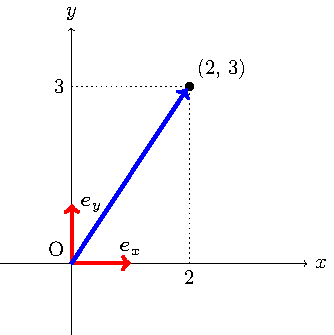
\includegraphics[width=5.5cm]{picture/vecter8.pdf}
 \caption{直交直線座標系における標準基底}
 \end{center}
\end{figure}

さて,この座標系に対応するような基底の取り方というのはもちろん標準基底のことである.
例えば点$(2, \, 3)$といえば,これは原点から右向きに2,上向きに3だけ進んだような点を表すのだった.
これはちょうど位置ベクトル$\left[ 
\begin{array}{c}
2 \\
3
\end{array}
\right] $に相当し,このベクトルは標準基底$ \{ \, \bm{e}_x, \, \bm{e}_y \, \} $を使えば
$2\bm{e}_x+3\bm{e}_y$と表せるのであった.さっきまでと標準基底の添え字の使い方を変えているが,
これは$xy$平面という言葉に引きずられてそうなっている.

この座標系を考案したのはDescartesという人物である.
そういうわけで,直交直線座標系のことを\textbf{Descartes座標系}
\index[widx]{ざひょうけい@座標系!Descartes@Descartes---}
\index[nidx]{Descartes@Descartes(デカルト)}
と呼ばれることも多い.人名が付いた用語というのはなんとなくかっこいいものである.
英語圏では``Descartesの''という意味を表す形容詞としてCartesian(カーテシアン)
という用語がある.そういうわけで,海外での生活が長い人などはDescartes座標系ではなく
\textbf{Cartesian座標系}
\index[widx]{ざひょうけい@座標系!Cartesian@Cartesian---|see{Descartes座標系}}
などと呼ぶこともあるそうだ.

\subsubsection{斜交直線座標系}
座標系の取り方はもちろんDescartes座標系だけではない.
``直交直線座標系''というところから``直交''という要素を取り払ってみよう.

座標軸の引き方は,さっきと同じく直線を2本引くのだが,
この線の引き方は平行でもなければもはや自由である.
線の引き方表現するかについてであるが,
引いた直線と同じ向きのベクトルを2本用意してみよう.
そして,$\bm{a}$方向と$\bm{b}$方向に直線を引き,その2本の直線を座標軸としてみる.
例えばそれを$\bm{a}, \, \bm{b}$として,``私は$\bm{a}$方向と$\bm{b}$方向を軸にします''といっておけばいいのである.
こういう場合,引いた直線のことを$\bm{a}$軸,$\bm{b}$軸などというように呼ぶこともある.
$\bm{a}$と$\bm{b}$はもちろん線形独立で,$\mathbb{R}^2$の基底になる.
そして,平面上のベクトルを$\bm{a}$と$\bm{b}$の線形結合で表したときの係数がそのベクトルの
基底$\{ \, \bm{a}, \, \bm{b} \, \} $に関する座標ということになる.
すなわち,$\bm{a}, \, \bm{b}$という2本のベクトルを用意することにより,
座標を決定するための規則,つまり座標系が与えられたことになる.
このように,直交せず,かつ平行でない2本の直線を基準とした座標系を
\emph{斜交直線座標系}\index[widx]{ざひょうけい@座標系!しゃこうちょくせん@斜交直線---}と呼ぶ.

例を出して考えてみよう.Descartes座標系で表したときの成分表示が$\left[
\begin{array}{c} 
\displaystyle \frac{1}{4} \\
1
\end{array} 
\right]$
になるようなベクトルを$\bm{a}$,
$\left[
\begin{array}{c}
1 \\ 
\displaystyle \frac{1}{4} 
\end{array} 
\right]$
になるようなベクトル$\bm{b}$を考え,これらを基準とした斜交直線座標系を導入する.
この座標系における座標が$\left( \displaystyle \frac{8}{3}, \, \frac{4}{3} \right)$
となるような点の様子は図\ref{fig:syakou}
のようになる.
\begin{figure}[h]
 \begin{center}
 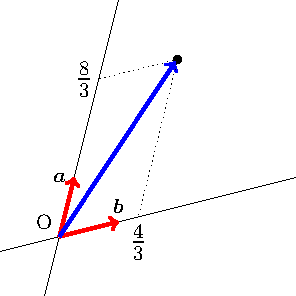
\includegraphics[width=4.8cm]{picture/vecter9.pdf}
 \caption{斜交直線座標系とその基底}
\label{fig:syakou}
 \end{center}
\end{figure}
\\
この座標系における座標が$\left( \displaystyle \frac{8}{3}, \, \frac{4}{3} \right)$
となるような点に対応する位置ベクトルは
$ \displaystyle \frac{8}{3} \bm{a} + \frac{4}{3} \bm{b} $と書き表されるというわけだ.
この点をDescartes座標系で表すとどうなるだろうか? これはとても簡単で,
$\bm{a}$と$\bm{b}$をDescartes座標系で表してやって計算すればいいのであり,
\begin{align*}
\frac{8}{3} \bm{a} + \frac{4}{3} \bm{b} & = \frac{8}{3} \left( \frac{1}{4} \bm{e}_x + 1 \bm{e}_y \right)
+ \frac{4}{3} \left( 1 \bm{e}_x + \frac{1}{4} \bm{e}_y \right) \\
& = \frac{2}{3} \bm{e}_x + \frac{8}{3} \bm{e}_y + \frac{4}{3} \bm{e}_x +\frac{1}{3} \bm{e}_y \\
& = 2 \bm{e}_x + 3 \bm{e}_y
\end{align*}
となって,この点の座標をDescartes座標系で表すと$(2, \, 3)$となるということがわかる.
つまり,さっきの座標系で座標が$\left( \displaystyle \frac{8}{3}, \, \frac{4}{3} \right) $となるような点と,
Descartes座標系で座標が$(2, \, 3)$となるような点は同じ点なのだ.
座標系を変えれば点を表す座標も変わるのである.
このことには注意を払わねばなるまい.しかし,通常は点$(2, \, 3)$といえば,
これはDescartes座標系での座標が$(2, \, 3)$であるような点を表す.
違う座標系を用いるときはその都度断るのが原則である.
この文章もそういうように気を付けて書いてあるはずだ.

基底$\{ \, \bm{e}_x, \, \bm{e}_y \, \} $から基底$ \{ \, \bm{a}, \, \bm{b} \, \} $の変換行列を求めてみよう.
$\bm{a}$と$\bm{b}$は$\bm{e}_x, \, \bm{e}_y$を用いて
\begin{align*}
\bm{a} & = a_x \bm{e}_x + a_y \bm{e}_y \\
\bm{b} & = b_x \bm{e}_x + b_y \bm{e}_y
\end{align*}
と表せる.本当は$a_x$や$b_y$などといった値はわかっているのだが,
いまは式を一般的に考えるためにあえて値を文字にしている.
この式から,2次の正方行列$P$を
\begin{align*}
P= 
\left[
\begin{array}{cc}
a_x & b_x \\
a_y & b_y 
\end{array}
\right]
\end{align*}
と定めれば,
\begin{align*}
\left[
\begin{array}{cc}
\bm{a} & \bm{b} 
\end{array}
\right]
=
\left[
\begin{array}{cc}
\bm{e}_x & \bm{e}_y
\end{array}
\right]
P
\end{align*}
という関係式が成り立っていることになる. 
つまり,基底$\{ \, \bm{e}_x, \, \bm{e}_y \, \} $から基底$ \{ \, \bm{a}, \, \bm{b} \, \} $の変換行列$P$は
\begin{align*}
P=
\left[
\begin{array}{cc}
\bm{a} & \bm{b}
\end{array}
\right]
\end{align*}
ということになる.ちょうど基底を2本並べた形になっている.
この行列$P$は基底同士の関係を表す行列である.

ところで,我々が普段目にしているのは座標同士の関係式である.
それを求めてみよう.

Descartes座標系での座標が$(x, \, y)$になるような点の位置ベクトルを$\bm{r}$とする.
$\bm{r}$を$\bm{a}, \, \bm{b}$というベクトルを基準とした斜交直線座標系で表したときに,
その座標が$(x', \, y')$になったとする.$x, \, y$と$x', \, y'$の関係式を求めたい.
$\bm{a}, \, \bm{b}$は標準基底を用いて
\begin{align*}
\bm{a} & = a_x \bm{e}_x + a_y \bm{e}_y \\
\bm{b} & = b_x \bm{e}_x + b_y \bm{e}_y
\end{align*}
と書き表せるとしよう.$\bm{r}$をそれぞれの座標系で表すと
\begin{align*}
\bm{r} & = x \bm{e}_x + y \bm{e}_y \\
\bm{r} & = x' \bm{a} + y' \bm{b} 
\end{align*}
となる.この式で$\bm{r}$は同じ1つのベクトルなので
\begin{align*}
x' \bm{a} + y' \bm{b} = x \bm{e}_x + y \bm{e}_y 
\end{align*}
となる.ここから$\bm{a}, \, \bm{b}$を消去してやると
\begin{align*}
x' ( a_x \bm{e}_x + a_y \bm{e}_y ) + y' ( b_x \bm{e}_x + b_y \bm{e}_y ) & = x \bm{e}_x + y \bm{e}_y \\
\therefore (a_x x' + b_x y' ) \bm{e}_x  + ( a_y x' + b_y y' ) \bm{e}_y & = x \bm{e}_x + y \bm{e}_y
\end{align*}
標準基底$\bm{e}_x, \, \bm{e}_y$はもちろん線形独立であるから
\begin{align*}
a_x x' + b_x y' & = x \\
a_y x' + b_y y' &= y
\end{align*}
ということになる.さっきの行列$P$を使ってみると
\begin{align*}
P 
\left[
\begin{array}{c}
x' \\
y'
\end{array}
\right]
= 
\left[
\begin{array}{c}
x \\
y
\end{array}
\right]
\end{align*}
となる.$P$の逆行列$P^{-1}$を用いれば
\begin{align*}
\left[
\begin{array}{c}
x' \\
y' 
\end{array}
\right]
= P^{-1}
\left[
\begin{array}{c}
x \\
y
\end{array}
\right]
\end{align*}
という関係式が得られる.
この行列$P^{-1}$は座標同士の関係を表す行列である.
行列の逆行列というのは存在しない可能性があるのだが,
基底を変換するような行列であれば問題ないことがわかっている.
イメージとしても明らかである.もし$P^{-1}$が存在しなかったときのことを考えてみればすぐにわかるはずだ.
もしこの式を基底同士の関係式と同じ形式で書きたければ,両辺の転置行列をとって
\begin{align*}
\left[
\begin{array}{cc}
x' & y' 
\end{array}
\right]
= 
\left[
\begin{array}{cc}
x & y 
\end{array}
\right]
{}^t\!P^{-1}
\end{align*}
としてやればいい.${}^t$は転置行列を表す記号である.
流儀によっては行列の右上に${}^\top$という記号を置いて転置行列を表すこともある.
座標同士の関係式と基底同士の関係式とで
用いる行列が違うのがわかるだろうか? 座標変換で混乱するのは大体このあたりである.
何についての関係式なのかをきちんと追わないとよくわからないことになってしまうので注意しよう.

\begin{itembox}[l]{検討}
行列$P$について,${}^t \! P ^{-1} =P$が成り立つのは$P$がどんな行列のときだろうか? また,そのときの$P$
はどんな座標変換を表すだろうか? 
\end{itembox}

\subsubsection{極座標系}
次に,極座標系という座標系について考えてみる.
おそらく,直交直線座標系以外の座標系で,高校数学で初めて明示的に登場するものが極座標である.
\footnote{明示的にではないが,数学Bで斜交直線座標系は登場している.}
極座標系においては,まず座標同士の関係式を導いてから基底同士の関係式に移ることにする.
これは,非常に特殊な事情があってそうすることにした.理由は後になればいやというほどわかるだろう.

極座標系においては,まず平面上に1点Oをとり,さらにO以外の点を1つとり,これをXとする.
この点Oのことを\emph{極}\index[widx]{きょく@極}といい,半直線OXのことを\emph{始線}
\index[widx]{しせん@始線}という.

さて,平面上の点Pが与えられたとき,2点O,Pの距離を$r$とし,直線OPと半直線OXのなす角を$\theta$とする.
OXは半直線であって向きが存在することに注意しよう.
このときの$\theta$を点Pの\emph{偏角}\index[widx]{へんかく@偏角}という.
また,半直線OPのことを点Pの\emph{動径}\index[widx]{どうけい@動径}と呼ぶ.

このとき,ただ1点Oを除いては平面の各点に対して$r$と$\theta$はただ1つに定まり,
$\theta$が$0 \leq \theta < 2 \pi$であるとすれば,各$r$と$\theta$に対してそれに対応する点もただ1つに定まる.
$r$と$\theta$がまったく同じであるような異なる2点というのは明らかに存在しないだろう.
ゆえに,極というただ1点を除いては,
平面上の点の位置というのは$r$と$\theta$によって完全に定めることができるのである.
これはすなわち,平面上の点の位置を決定するためのルールが与えられたことになり,
座標系を導入したことに相当するわけだ.
極においては$r=0$であるが$\theta$は決定できない.しかしそんな細かいことはこの際無視することにする.
2点O,Pの距離が$r$で,直線OPと半直線OXのなす角が$\theta$であったとき,
点Pの座標は$( r, \, \theta )$であるとしよう.
このような座標系が\emph{極座標系}\index[widx]{ざひょうけい@座標系!きょく@極---}である.
\begin{figure}[h]
 \begin{center}
 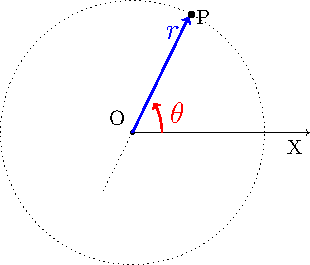
\includegraphics[width=5cm]{picture/vecter10.pdf}
 \caption{極座標系における座標の決定}
\label{fig:kyokuzahyou}
 \end{center}
\end{figure}

極座標系が直交直線座標系や斜交直線座標系とはちょっと趣の違った座標系であることが見て取れるだろう.
``座標''という用語を位置ベクトルを基底の線形結合で表したときの係数であると定義したが,
今回は基底とは独立に座標を定義している.
極座標系における基底はその座標をもとに定義されるのである.
このことに関しては後で話そうと思う.

そういえば,極座標系について説明するにあたり,$\theta$の範囲を制限したが,
実際にはそんなことをしない方がいろいろと便利である.
例えば,極座標系においての座標が$ \displaystyle \left(1, \, \frac{7}{4} \pi \right)$ となるような点と,
座標が$\displaystyle \left(1, \, - \frac{\pi}{4} \right)$となるような点は同じ点であるとみなすのである.
こうしてしまうと$r, \, \theta$の組と平面上の点が1対1に対応しなくなってしまう.
しかし,そんな細かいことは無視することにするのである.
こうすることで何がどのように便利になるかはけっこういろいろあるので自身で考えてみるといいだろう.

\begin{figure}[h]
 \begin{center}
 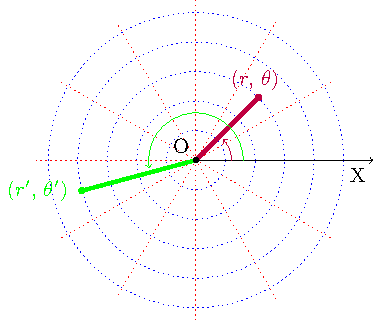
\includegraphics[width=6cm]{picture/vecter11.pdf}
 \caption{極座標系は直交曲線座標系である}
\label{fig:kyokukyokusen}
 \end{center}
\end{figure}

2次元のDescartes座標系においては,基準にしたのは2本の直交する直線であり,
斜交直線座標系においては,直交せず平行でない2本の直線であった.
では,極座標系においては何が基準になっているのだろう? 答えは図\ref{fig:kyokukyokusen}に
それとなく書いてあるのだが,それは円と直線である.
平面上に極を中心とする無数の円を描く.中心が決まっているのでそれらの円を特徴づけるのは半径である.
平面上に点が与えられたとき,その点と極との距離と同じ半径の円上にその点は存在していることになる.
つまり,点に与えられる座標のうち$r$の部分は,その点がどの円に属しているかを表すのである.
また,平面上に極を通る直線を無数に描く.通る点が1つ決まっているのでそれらの直線は
通る点をもう1つ決めることによって特徴づけることもできるが,違う特徴づけもできる.
それは,その直線とOXのなす角である.これは,ちょうど点の偏角$\theta$に相当しているのがわかるだろう.
すなわち,点に与えられる座標のうち偏角$\theta$に当たる部分は,
その点がどの直線に属しているかを表しているのである.

極座標系が極を通る直線と極を中心とする円を基準にしていることがわかるだろう.
そして,円と直線は互いにすべて直交している.
従って,極座標系は\emph{直交曲線座標系}\index[widx]{ざひょうけい@座標系!ちょっこうきょくせん@直交曲線---}
と呼ばれることもある.
しかし,直交曲線座標系が極座標系しかないというわけではない.
直交する曲線を用いるような座標系はすべて直交曲線座標系と呼ばれるからだ.
また,極座標系は曲線の中でも円を使っている.
そういうわけで,
2次元の極座標系は\emph{円座標系}\index[widx]{ざひょうけい@座標系!えん@円---|see{極座標系}}とも呼ばれる.
2次元のとわざわざ書いたのは,3次元だと違う呼ばれ方をするからだ.
そのことに関してはそのときに触れることにしよう.

さて,極座標系とDescartes座標系との関係を見てみよう.
結果から言うと,Descartes座標系での座標が$(x, \, y)$,
極座標系での座標が$(r, \, \theta)$であるような点において,
三角関数の定義により次の関係式が成り立っているといえる.
\begin{align}
\begin{aligned}
x & = r \cos \theta \\
y & = r \sin \theta 
\label{eq:kyokuhenkan}
\end{aligned}
\end{align}
もちろん,Descartes座標系での座標軸と始線と極をうまい具合にとらないと
こういうきれいな関係式は成り立たない.
具体的には,Descartes座標系での原点を極座標系での極とし,
Descartes座標系での$x$軸を極座標系での始線とするのである.
\begin{figure}[h]
 \begin{center}
 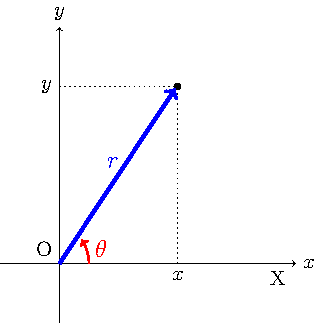
\includegraphics[width=5cm]{picture/vecter12.pdf}
 \caption{極座標系とDescartes座標系}
\label{fig:kyokuDescartes}
 \end{center}
\end{figure}

こうして見ると,極座標系における始線をOXと書いた理由がなんとなくわかる気がする.
始線OXと$x$軸が対応するようになっていたというわけだ.
原点と極,そして始線と$x$軸が一致しないようにして式(\ref{eq:kyokuhenkan})が破綻するように
することもできるのだが,この美しくわかりやすい関係式を捨てるという選択肢をとることはまずあるまい.
そういうわけで,極座標系を式(\ref{eq:kyokuhenkan})が成り立つような座標系というように定義している本はけっこう多い.
もちろんそれで間違っているわけではないのだが,極座標系というのはDescartes座標系
とはまったく独立に定義できるのだということ伝えたかったので,今回のような定義の仕方をしたのだった.

座標同士の関係式が終わったところで,いよいよ基底同士の関係式を求めてみよう.
斜交直線座標系での話を思い出してほしい.
それによれば,平面上の点について,
ある座標系における座標が$(x, \, y)$であり,別の座標系における座標が$(x', \, y')$
であるとき,それらの関係は行列$P$を用いて
\begin{align*}
\left[
\begin{array}{cc}
x' & y'
\end{array}
\right]
=
\left[
\begin{array}{cc}
x & y
\end{array}
\right]
{}^t \! P^{-1}
\end{align*}
というように表せるのであった.
いまはDescartes座標系と極座標系について考えているので
\begin{align*}
\left[
\begin{array}{cc}
r & \theta
\end{array}
\right]
=
\left[
\begin{array}{cc}
x & y
\end{array}
\right]
{}^t \! P^{-1}
\end{align*}
という関係式が成立するような行列$P$を探すことになる.
賢明な読者の方は気づいたはずだが,
そんな行列$P$はどう頑張っても見つからないのである.
なぜだろうか? 今までの議論のどこがに間違いがあったのだというのだろうか? 本当はこういうことについてじっくり悩むのは
とても有益なことなのだが,さっさと先に進んでしまいたいので結論を言ってしまおう.
すべての座標変換が行列を使って表せるわけではないのである.
行列を使って表せるような座標変換は\emph{線形変換}\index[widx]{せんけいへんかん@線形変換}と呼ばれ,
とても面白い性質を持った変換である.だが,性質のいい座標変換はこれだけではないのである.
斜交直線座標系は,たまたまDescartes座標系に
線形変換を施すことによって得られる座標系であったということだ.
だが今回は違うのである.違ったアプローチをする必要がありそうである.

そういえば,``極座標系における基底''とはいったいなんだろうか? Descartes座標系における基底は
標準基底のことで,斜交直線座標系における基底というのは引いた2本の直線と同じ向きのベクトルのことであった.
それに対して,``極座標系における基底''というのはいまいちイメージがつかない.
極座標系というのは円と直線を基準に据えているのであった.
これまでの話からすると,円と直線の向きに沿った2本のベクトルをとり,
それを極座標系における基底とするのだろう.
しかし,極座標系においては,直線といっても向きの違う直線が無数にあるし,
円の向きに沿ったベクトルなどという言葉は最早意味不明である.
意味不明なら定義してしまえばいい.よくわからない,
曖昧なものはきちんと定義して明確にしてしまえばいいのである.

とはいっても,どう定義したらいいだろうか.いままでの定義の方法は使えないが,
できれば同じような定義の方法を使いたいものである.
平面上において,ある1点Pを考える.極座標系においては点Pの座標は$(r, \, \theta)$であるとしておこう.
半直線OPの方向に大きさ1のベクトルをとり,これを$\bm{e}_r$とする.
そして,点Pが属している円の点Pにおける接線に平行な大きさ1のベクトルを
角度$\theta$を測った向きにとり,これを$\bm{e}_\theta$としておく.

各$r, \, \theta$について,$\bm{e}_r$と$\bm{e}_\theta$の長さは1で,しかも直交している.
もちろん,$ \{ \, \bm{e}_r, \, \bm{e}_\theta \, \} $は2次元平面$\mathbb{R}^2$の基底になっている. 
なんとなく標準基底と似ている気がするが,決定的に違う点が1つある.
それは,基底のとり方が座標に依存しているということだ.
いままでの座標系においては,基底は座標に依存することはなかった.
Descartes座標系においては標準基底$\bm{e}_x = 
\left[
\begin{array}{c}
1 \\
0
\end{array}
\right]
, \, 
\bm{e}_y =
\left[
\begin{array}{c}
0 \\
1
\end{array}
\right]$
であったし,斜交直線座標系においても定まった2本のベクトルをまず用意し,
それを使って平面上の点の位置を決めていたのであった.
しかし,いまとった基底に関しては,各点に対して1組ずつ基底が与えられており,
各点ごとにそれぞれの基底を用いるというイメージになっている.
\begin{figure}[h]
 \begin{center}
 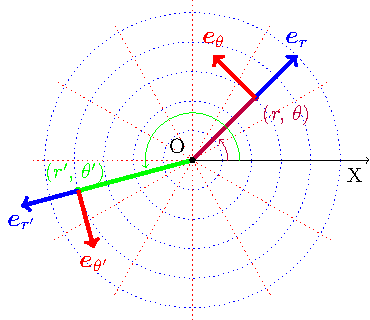
\includegraphics[width=6.5cm]{picture/vecter13.pdf}
 \caption{極座標系における基底のとり方}
\label{fig:kyokukitei}
 \end{center}
\end{figure}
\\
図\ref{fig:kyokukitei}において,
図中の点$(r, \, \theta)$と点$(r', \, \theta')$には違う基底が対応しているのが見て取れる.
しかし,$r$だけが変化してもそれに対応する基底は変化しない.
いまはわかりやすいように各点を始点にしてその点に対応する基底を描いているが,
平行移動して重なるようなベクトルは同じものとみなすからである.

ここまでやると,自分がこれからやろうとしていたことが少し変わっていることに気づく.
いままでは極座標系における定まった基底(そんなものはとれなかったが)と標準基底との関係を求めたかったのだが,
いまからやるのは極座標系において,点$(r, \, \theta)$に対応する基底$\{ \, \bm{e}_r, \, \bm{e}_\theta \, \} $と
標準基底との関係を求めることである.
ここまで引っ張ってしまって申し訳ないのだが,実はこの関係を求める作業は一瞬で終わってしまうのである.
結論だけ先に述べよう.
極座標系において,点$(r, \, \theta)$に対応する基底$\{ \, \bm{e}_r, \, \bm{e}_\theta \, \} $と
標準基底$\{ \, \bm{e}_x, \, \bm{e}_y \, \}$との関係は次の通りである.
\begin{align}
\begin{aligned}
\bm{e}_r& = & \cos \theta \, \bm{e}_x & & + \sin \theta \, \bm{e}_y & \\
\bm{e}_\theta & = &  - \sin \theta \, \bm{e}_x & & + \cos \theta \, \bm{e}_y &
\label{eq:kyokukiteihenkan}
\end{aligned}
\end{align}
わからない人は次の図\ref{fig:kyokukiteikankei}を3年ほどじっくり眺めてほしい.
\begin{figure}[h]
 \begin{center}
 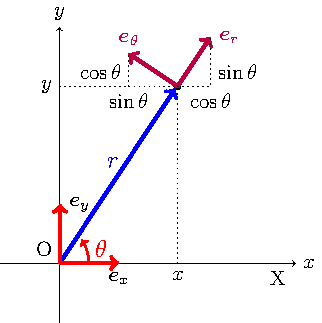
\includegraphics[width=5cm]{picture/vecter14.pdf}
 \caption{極座標系における基底と標準基底との関係}
\label{fig:kyokukiteikankei}
 \end{center}
\end{figure}
\\
これでもわからない人にヒントを出すと,$\bm{e}_r$というのは大きさが1だから,
図\ref{fig:kyokukiteikankei}を見ると,始点から大きさ$\cos \theta$だけ$\bm{e}_x$方向に進み,ついで
大きさ$\sin \theta$だけ$\bm{e}_y$方向に進むとちょうど$\bm{e}_r$の終点にたどり着くことになる.
これはつまり,$\bm{e}_r=\cos \theta \, \bm{e}_x + \sin \theta \, \bm{e}_y$が成り立つということである.
そうそう,もし``大きさ''と書いた量が負であれば,
それは``・・・方向に''というところを逆向きに進むのだと解釈してほしい.
面倒なので以後,こういった注釈は述べないことにする.

$\bm{e}_\theta$も同じように考えて,まず大きさ$\sin \theta$だけ$-\bm{e}_x$方向に進み,
さらにそこから大きさ$\cos \theta$だけ$\bm{e}_y$方向に進むことで$\bm{e}_\theta$の終点にたどり着くのである.
従って$\bm{e}_\theta = - \sin \theta \, \bm{e}_x + \cos \theta \, \bm{e}_y$が成り立つ.
ベクトルの和と三角関数の定義が頭に入っていればできてしまう簡単な作業である.
ここまであからさまなヒントを出せばできるだろう.式(\ref{eq:kyokukiteihenkan})において,
行列$P$を
\begin{align*}
P = \left[
\begin{array}{cc}
\cos \theta & -\sin \theta \\
\sin \theta & \cos \theta
\end{array}
\right]
\end{align*}
と定めれば,式(\ref{eq:kyokukiteihenkan})は
\begin{align*}
\left[
\begin{array}{cc}
\bm{e}_r & \bm{e}_\theta 
\end{array}
\right]
=
\left[
\begin{array}{cc}
\bm{e}_x & \bm{e}_y
\end{array}
\right]
P
\end{align*}
と書き換えられる.基底$\{ \, \bm{e}_x , \, \bm{e}_y \, \} $
から基底$\{ \, \bm{e}_r , \, \bm{e}_\theta \, \}$への変換行列はいま定義した$P$であるというわけだ. 

本当はもう少し伝えておきたいことはあるのだが,それはまた別の機会にして先に進むことにしよう.

\subsection{3次元空間における座標系}
これからやるのは3次元空間における座標系である.
よく3次元空間は``縦+横+高さ''と言われることがあるがそうではない.
これは,次元の概念を説明するときに触れたのだった.
とはいえ,このイメージはそこそこ役に立つものである.
ここでは,2次元平面での座標に対してさらにもう1個座標を追加することによって
3次元空間における座標系を構成してみよう.
\subsubsection{3次元直交直線座標系}\index[widx]{ざひょうけい@座標系!Descartes@Descartes---}
Descartes座標系から始めよう.
2次元のDescartes座標系では平面上に引かれた2本の直交する直線が基準であった.
3次元のDescartes座標系であれば,ここに直線を1本追加してやればいい.
直交直線座標系というだけあって,
加える直線はもともと引いてあった直線の両方に直線に直交するように引くことになる.

2次元のDescartes座標系においては,
平面に引かれた2本の直線はそれぞれ$x$軸,$y$軸と呼ばれるのであった.
そのつながりで,新たに引いた直線は\emph{$z$軸}と呼ばれるのが普通である.
$x$軸,$y$軸,$z$軸の3本の直線が空間内の座標を決定するルールの象徴になっている.
そういうわけで,Descartes座標系が導入された3次元空間は\emph{$xyz$空間}
と呼ばれることがある.
基底としては,3次元数ベクトル空間$\mathbb{R}^3$における
標準基底$\{ \, \bm{e}_1, \, \bm{e}_2, \, \bm{e}_3 \, \}$をそのまま持ってくればいい.
これらの標準基底は$xyz$空間の各軸に沿った大きさ1のベクトルになっている.
添え字を変えて$\{ \, \bm{e}_x, \, \bm{e}_y, \, \bm{e}_z \, \}$としておこう.

ところで,紙に$xyz$空間を描いてみると,
どうやら軸の引き方によって2種類の異なる座標系が出来上がるようなのだ.
\begin{figure}[h]
 \begin{minipage}{0.5\hsize}
  \begin{center}
   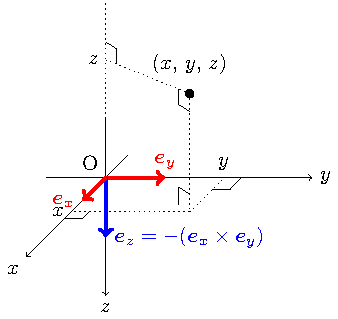
\includegraphics[width=5cm]{picture/vecter16}
  \end{center}
 \caption{左手系}
\label{fig:hidaritekei}
\end{minipage}
\begin{minipage}{0.5\hsize}
  \begin{center}
   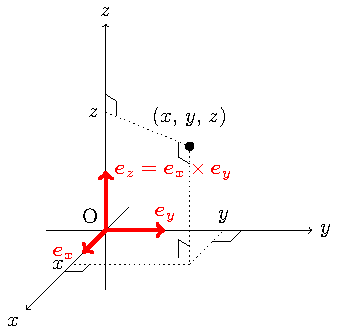
\includegraphics[width=5cm]{picture/vecter15}
  \end{center}
 \caption{右手系}
\label{fig:migitekei}
\end{minipage}
\end{figure}
\\
右と左に書いてある2つの座標系が違うのがわかるだろうか? 右(図\ref{fig:migitekei})に書いてある座標系は
\emph{右手系}\index[widx]{みぎてけい@右手系},
左(図\ref{fig:hidaritekei})に書いてある座標系は
\emph{左手系}\index[widx]{ひだりてけい@左手系}と呼ばれている.
右手系,左手系という言葉は本当はもう少し広い意味で使われているのだが,
ここでは省略させてもらうことにする.
両座標系を比較すると,$z$軸が逆向きに引かれているのがわかるだろう.
この2つの座標系はいくら回転させても重ね合わせることはできない.
ちょうど右手と左手の関係になっているというわけだ.

さて,普通Descartes座標系といえば図\ref{fig:migitekei}にある
右手系が業界標準である.
右手系においては$\bm{e}_z=\bm{e}_x \times \bm{e}_y$が成り立っているが,
左手系において成り立っているのは$\bm{e}_z = -( \bm{e}_x \times \bm{e}_y )$である.

演習として,次に示す4つの座標系がそれぞれ右手系であるか左手系であるか判定してみてほしい.
\begin{figure}[h]
 \begin{minipage}{0.5\hsize}
  \begin{center}
   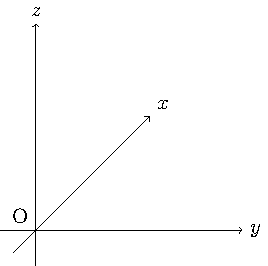
\includegraphics[width=3.5cm]{picture/vecter17}
  \end{center}
\end{minipage}
\begin{minipage}{0.5\hsize}
  \begin{center}
   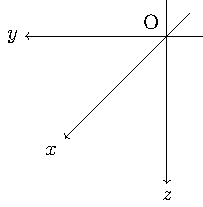
\includegraphics[width=3.5cm]{picture/vecter18}
  \end{center}
\end{minipage}
\end{figure}
\\
\begin{figure}[h]
 \begin{minipage}{0.5\hsize}
  \begin{center}
   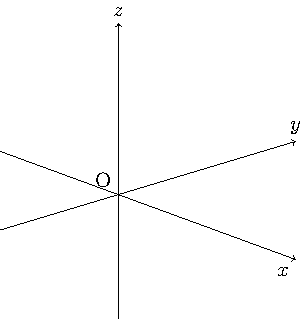
\includegraphics[width=3.7cm]{picture/vecter19}
  \end{center}
\end{minipage}
\begin{minipage}{0.5\hsize}
  \begin{center}
   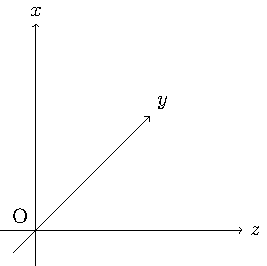
\includegraphics[width=3.5cm]{picture/vecter20}
  \end{center}
\end{minipage}
\end{figure}

\subsubsection{3次元斜交直線座標系}\index[widx]{ざひょうけい@座標系!しゃこうちょくせん@斜交直線---}
直交直線座標系の次は斜交直線座標系である.
といっても,Descartes座標系ほど語ることは多くはない.
さっさと進んでしまうことにしよう.

線形独立であるようなベクトルを3つとり,
これを$\mathbb{R}^3$の基底としてみる.
ここではそれを$\bm{a}, \, \bm{b}, \, \bm{c}$としてみよう.
ただし,これらのベクトルは直交しているわけではない.
大きさも1である必要はない.
この基底の取り方の自由さこそが斜交直線座標系の利点である.
$\bm{a}, \, \bm{b}, \, \bm{c}$の成分表示を
\begin{align*}
\bm{a} = \left[
\begin{array}{c}
a_x \\
a_y \\
a_z
\end{array}
\right]
\; , \;  \;
\bm{b} = \left[
\begin{array}{c}
b_x \\
b_y \\
b_z
\end{array}
\right]
\; , \;  \;
\bm{c} = \left[
\begin{array}{c}
c_x \\
c_y \\
c_z
\end{array}
\right]
\end{align*}
としてみる.
これらのベクトルは標準基底を用いて
\begin{align*}
\bm{a} & = a_x \bm{e}_x + a_y \bm{e}_y + a_z \bm{e}_z \\
\bm{b} & = b_x \bm{e}_x + b_y \bm{e}_y + b_z \bm{e}_z \\
\bm{c} & = c_x \bm{e}_x + c_y \bm{e}_y + c_z \bm{e}_z 
\end{align*}
と表せる.
よって,行列$P$を
\begin{align*}
P = \left[
\begin{array}{ccc}
a_x & b_x & c_x \\
a_y & b_y & c_y \\
a_z & b_z & c_z 
\end{array}
\right]
\end{align*}
と定めると,
\begin{align*}
\left[
\begin{array}{ccc}
\bm{a} & \bm{b} & \bm{c} 
\end{array}
\right]
= 
\left[
\begin{array}{ccc}
\bm{e}_x & \bm{e}_y & \bm{e}_z 
\end{array}
\right] P
\end{align*}
が成り立つ.ゆえに,標準基底$\{ \, \bm{e}_x , \, \bm{e}_y , \, \bm{e}_z \, \}$から
基底$\{ \, \bm{a} , \, \bm{b} , \, \bm{c} \, \}$への変換行列はこの$P$ということになる.
これは,以前も話した内容である.
\subsubsection{スカラー三重積とベクトル三重積}
書くことが少なくて寂しいのでちょっと寄り道をしてみよう.
$\bm{a}, \, \bm{b}, \, \bm{c}$の3本のベクトルの線形結合全体を考えると,
もちろんもとのベクトル空間である$\mathbb{R}^3$を再現する.
しかし,$\bm{a}, \, \bm{b}, \, \bm{c}$自体は,平行六面体を構成する.
これを``$\bm{a}, \, \bm{b}, \, \bm{c}$が張る平行六面体''と呼ぶことがある.
そして,その体積$V$は
\begin{align}
V = \bm{a} \cdot ( \bm{b} \times \bm{c} ) 
\label{eq:heikourokuV}
\end{align}
と表される.
このままだと$V$が負になることもあり,絶対値を付けておくべきである.
しかし式を簡単にするため,この$V$を符号付き体積とでも呼んでおくことにしよう.
\begin{figure}[h]
 \begin{center}
 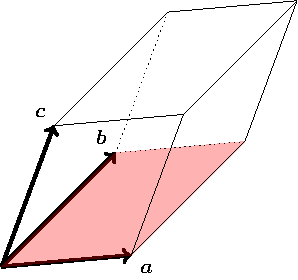
\includegraphics[width=4.5cm]{picture/vecter21.pdf}
 \caption{3つのベクトルが張る平行六面体}
\label{fig:heikourokumentai}
 \end{center}
\end{figure}
\\
図\ref{fig:heikourokumentai}中の色を付けた部分の面積が
$ \lvert \bm{a} \times \bm{b} \rvert $となることや
$ \bm{a} \cdot ( \bm{b} \times \bm{c} )$がスカラー量であることに納得がいき,
かつそれぞれの量が何を表しているかを考えられれば式(\ref{eq:heikourokuV})が
成り立つことは簡単に理解できるはずだ.
もしわからなければ,それは内積,外積の意味が理解できていないか,
もしくは平行六面体がどのような立体か理解していないだけである.
まぁその辺に関しては各自復習することにして,式(\ref{eq:heikourokuV})
を眺めながら,$V$のどこを底面とみなしているかを考えてやる.
そして,どこを底面とみるかを変えてやって,$V$を求めてやると,
次のような式が成り立つことがわかるはずだ.
\begin{align}
\bm{a} \cdot ( \bm{b} \times \bm{c} ) = \bm{c} \cdot ( \bm{a} \times \bm{b})
= \bm{b} \cdot ( \bm{c} \times \bm{a} ) 
\label{eq:sanjuuseki}
\end{align}
非常に対称的で美しい関係式である.
式(\ref{eq:sanjuuseki})中の \\
$\bm{a} \cdot ( \bm{b} \times \bm{c} ) , \, 
\bm{c} \cdot ( \bm{a} \times \bm{b}) , \, 
\bm{b} \cdot ( \bm{c} \times \bm{a} ) $
は$\bm{a}, \, \bm{b}, \, \bm{c}$の
\emph{スカラー三重積}\index[widx]{すからー@スカラー!さんじゅうせき@---三重積}と呼ばれている.
いまは線形独立である3つのベクトルについて考えたが,式(\ref{eq:sanjuuseki})は
$\bm{a}, \, \bm{b}, \, \bm{c}$が線形従属である場合にも成り立つ.
線形従属であるようなベクトル$\bm{a}, \, \bm{b}, \, \bm{c}$に対しては,
$\bm{a}, \, \bm{b}, \, \bm{c}$が張る平行六面体はつぶれてしまい,$V=0$になるからだ.
もうちょっと詳しくいうと,$\bm{a}, \, \bm{b}, \, \bm{c}$が線形従属のとき,
これらのベクトルは同一平面上にあって,$ \bm{b} \times \bm{c} $と$\bm{a}$が垂直になり,
その内積は0になる.他のパターンでも同じことが言えることはすぐにわかるはずだ.

スカラー三重積というからにはベクトル三重積というのもある.
3つのベクトル$\bm{a}, \, \bm{b}, \, \bm{c}$について,
新しいベクトル$ \bm{a} \times ( \bm{b} \times \bm{c} ) , \, ( \bm{a} \times \bm{b} ) \times \bm{c}$
を$\bm{a}, \, \bm{b} , \, \bm{c}$の
\emph{ベクトル三重積}\index[widx]{べくとる@ベクトル!さんじゅうせき@三重積}と呼ぶ.
ここまでまじめに学習してきた読者なら,なぜ私が
$ \bm{a} \times ( \bm{b} \times \bm{c} ) , \, ( \bm{a} \times \bm{b} ) \times \bm{c}$
とわざわざ2つ書いたかわかるはずだ.これら2つのベクトルは同じベクトルであるとは限らない.
ベクトル三重積についての詳細は省略するが,次のような等式が成立することが知られている.
\begin{align}
\begin{aligned}
\bm{a} \times ( \bm{b} \times \bm{c} ) = 
( \bm{a} \cdot \bm{c} ) \bm{b} 
- ( \bm{a} \cdot \bm{b} ) \bm{c} \\
\bm{b} \times ( \bm{c} \times \bm{a} ) = 
( \bm{b} \cdot \bm{a} ) \bm{c} 
- ( \bm{b} \cdot \bm{c} ) \bm{a} \\
\bm{c} \times ( \bm{a} \times \bm{b} ) = 
( \bm{c} \cdot \bm{b} ) \bm{a} 
- ( \bm{c} \cdot \bm{a} ) \bm{b} \\
( \bm{a} \times \bm{b} ) \times \bm{c}  = 
( \bm{a} \cdot \bm{c} ) \bm{b} 
- ( \bm{b} \cdot \bm{c} ) \bm{a} \\
( \bm{b} \times \bm{c} ) \times \bm{a}  = 
( \bm{b} \cdot \bm{a} ) \bm{c} 
- ( \bm{c} \cdot \bm{a} ) \bm{b} \\
( \bm{c} \times \bm{a} ) \times \bm{b}  = 
( \bm{c} \cdot \bm{b} ) \bm{a} 
- ( \bm{a} \cdot \bm{b} ) \bm{c} \\
\label{eq:vecsanjuuseki}
\end{aligned}
\end{align}
式の多さに圧倒されそうだが,実は式(\ref{eq:vecsanjuuseki})
のうちどれか1つでも覚えておけば残りの式はそこから導くことができる.
一番上の式
\begin{align*}
\bm{a} \times ( \bm{b} \times \bm{c} ) = 
( \bm{a} \cdot \bm{c} ) \bm{b} 
- ( \bm{a} \cdot \bm{b} ) \bm{c}
\end{align*}
の$\bm{a}$を$\bm{b}$に,$\bm{b}$を$\bm{c}$に
置き換えてみると,
\footnote{え? ``置き換える''の意味が分からないって? ならば$\bm{a}, \, \bm{b}, \, \bm{c}$を
○,×,△とでも``置き換えて''みよ.}
2番目の式
\begin{align*}
\bm{b} \times ( \bm{a} \times \bm{b} ) = 
( \bm{b} \cdot \bm{a} ) \bm{c} 
- ( \bm{b} \cdot \bm{c} ) \bm{a}
\end{align*}
が導けるし,一番上の式と4番目の式を比較すると,これはちょうどかける順番が逆になっている.
外積においてかける順番を逆にするとどうなるかは以前話した通りである.
そんなこんなで同じようにしていけば残りの式も導くことができる.
まぁこの式をどこで使うかといわれると正直微妙なところはあるが.
式(\ref{eq:vecsanjuuseki})をよくよく眺めていると,
\begin{align}
\begin{aligned}
\bm{a} \times ( \bm{b} \times \bm{c} ) + \bm{b} \times ( \bm{c} \times \bm{a} ) + 
\bm{c} \times ( \bm{a} \times \bm{b} ) = \bm{0} \\
( \bm{a} \times  \bm{b} ) \times \bm{c} + ( \bm{b} \times  \bm{c} ) \times \bm{a} +
( \bm{c} \times  \bm{a} ) \times \bm{b} = \bm{0}
\label{eq:Jacobi}
\end{aligned}
\end{align}
という等式が成り立っていることに気が付くはずだ.
式(\ref{eq:Jacobi})は\textbf{Jacobiの恒等式}\index[widx]{Jacobiのこうとうしき@Jacobiの恒等式}
\index[nidx]{Jacobi@Jacobi(ヤコビ)}
と呼ばれているものの一部である.
一部というからには一般のものがあるわけなのだが,ちょっと説明がややこしいので省略させてもらおう.

ところで,3次元Descartes座標系のところで右手系と左手系というのが出てきたが,
スカラー三重積の知識があると,右手系,左手系という概念をもう少し一般に定義することができる.

3次元空間$\mathbb{R}^3$の基底を1組とり,これを$\Set{ \bm{a} , \, \bm{b} , \, \bm{c} }$
とする.$\bm{a} , \, \bm{b} , \, \bm{c}$
のスカラー三重積$\bm{a} \cdot ( \bm{b} \times \bm{c} )$
が正の値をとるとき,基底$\Set{ \bm{a} , \, \bm{b} , \, \bm{c} }$
は$\mathbb{R}^3$の\emph{右手系}\index[widx]{みぎてけい@右手系}をなすといい,
$\bm{a} \cdot ( \bm{b} \times \bm{c} )$
が負の値をとるとき,基底$\Set{ \bm{a} , \, \bm{b} , \, \bm{c} }$
は$\mathbb{R}^3$の\emph{左手系}\index[widx]{ひだりてけい@左手系}をなすという.

ぴったり直交しているわけではなくとも,
基底同士の向きの関係がDescartes座標系のときと
おおよそ同じようなものであればそれらを全部右手系とみなすのである.
Descartes座標系における標準基底$\Set{ \bm{e}_x , \, \bm{e}_y, \, \bm{e}_z }$
はもちろん$\mathbb{R}^3$の右手系をなしている.
これから学ぶ極座標系の基底もやはり$\mathbb{R}^3$の右手系をなす.
座標系は右手系を用いるのが業界標準なのである.

\subsubsection{3次元極座標系}\index[widx]{ざひょうけい@座標系!きょく@極---}
さて,お次は極座標系である.
極座標系においては基底ベクトルを増やしていくというアプローチは通用しない.
2次元極座標系においては,基底の代わりに幾何学的に座標を決定するルールを与えたのだった.
今回もその方法を利用していくことにする.

2次元極座標系のときに座標を決定するために用いたのは,
極を中心とする無数の円とそれに直交するような極を通る無数の直線であった.
3次元空間での点の座標を決定するには,ここにもうひとつ新たな要素を付け加えてやればいい.
ここでは,もうひとつ円を追加してやることにする.
この円は,極が中心で
かつ2次元極座標系のときの円と直線が存在した平面からは飛び出していることにしよう.
さらに,この円はもとの平面と直交しているという条件も付け加えてやる.
ここまで厳しい条件を付け加えないと使いやすい座標系は出来上がらないのだ.
もうひとつ円を追加すると書いたが,実際には上に書いたような条件をみたすような
円を無数に描くのだ.円の半径は特に指定してはいなかった.

2次元極座標系において,平面上の点が円上のどこにあるかを決定するのに,
始線とその点の動径のなす角を用いたのであった.
今回は円を追加したのだから,始線を追加してやればなんとかなりそうだ.
その始線をOZとしてみよう.空間内に点Zをとり,半直線OZを始線とするのである.
ただし,OZはOXと垂直であるということにしておく.

極と2本の始線によって,空間内の点の座標を定めよう.
我々に与えられたのは,極Oと直交する2本の半直線OX,OZである.
空間内に点Pがあったとする.まず2点O,Pの距離を求め,これを$r$とする.
次に,直線OPと半直線OZのなす角をはかり,これを$\theta$とおく.
そして,極Oを通り,OZに垂直な平面を考え,
極Oと,点Pからその平面に降ろした垂線の足の2点を通る直線を引く.
その直線と半直線OXのなす角を$\varphi$とする.
少し長くなったが,頭の中にイメージが思い浮かぶだろうか? 下の図と
自分が抱いていたイメージがおおむね一致するかをチェックしてほしい.
\begin{figure}[h]
 \begin{center}
 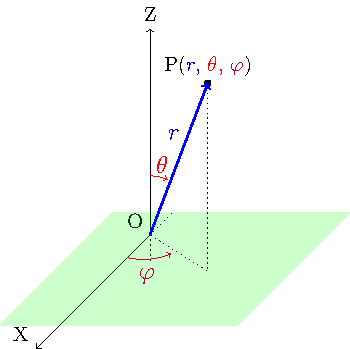
\includegraphics[width=5.7cm]{picture/vecter22.pdf}
 \caption{3次元極座標系における座標の決定}
\label{fig:3dkyokuzahyou}
 \end{center}
\end{figure}

空間内に与えられた点Pに対し,Pが直線OZ上になければ,$ r, \, \theta, \, \varphi $は必ず求めることができる.
そして,$r>0, 0 \leq \theta \leq \pi , \, - \pi < \varphi \leq \pi$とでもしておけば,
直線OZ上の点を除いては,各$r, \, \theta, \, \varphi$に対してそれに対応する点がただひとつ定まる.
そのとき,その点の座標は$(r, \, \theta, \, \varphi)$であると定義する.
直線OZ上の点に対しては$\varphi$を求めることができず,さらに極Oに関しては$\theta$も求めることができない.
だが,2次元極座標系のときと同じようにそんな細かいことは考えないことにする.
とにかく,これで空間内にある点の座標を定めるルールが決まったことになり,
無事に3次元極極座標系が定義されたことになる.

3次元極座標系における座標の決定は,極を通る無数の直線と,極を中心とする無数の円
によってなされるのであった.この円は,あらゆる方向に描かれている.
空間に点が与えられたとき,$r$がその点が属する円の半径を決め,
与えられた点が属する円がどの方向を向いた円かを$\varphi$が決定し,
$\theta$によってその円のどこに点が存在するかが決定されるのである.
しかし,あらゆる方向を向いた円が無数に存在している状況は,
その円と同じ半径の球が1つ存在している状況とまったく同じである.
円をその中心を通る軸周りに1回転して得られる
図形が球であることを思い出せば容易に納得できるだろう.
従って,3次元極座標系における座標の決定は,
極を通る無数の直線と,極を中心とする無数の球によってなされると考えることができるのである.
このイメージにおいては,空間に点が与えられたとき,まず$r$がその点が属する球の半径を決め,
その球のどこに点があるかを$\varphi, \, \theta$が決定するということになる.
この考え方でも座標の決定には何ら問題はなさそうである.
このことから,3次元極座標系は\emph{球面座標系}\index[widx]{ざひょうけい@座標系!きゅうめん@球面---},
もしくは\emph{球座標系}と呼ばれることがある.
なかなかよくできたネーミングである.

さて,ここからは3次元極座標系と3次元Descartes座標系との関係について考えてみる.
まずは座標同士の関係式だが,もはや何も言うまい.Descartes座標系における座標が
$(x, \, y, \, z)$であり,極座標系における座標が$(r, \, \theta, \, \varphi)$であるような点について,
以下のような関係式が成り立っている.
\begin{align}
\begin{aligned}
x & = r \sin \theta \cos \varphi \\
y & = r \sin \theta \sin \varphi \\
z & = r \cos \theta
\label{eq:kyokuDechenkan}
\end{aligned}
\end{align}
もちろん,これは式(\ref{eq:kyokuDechenkan})のような美しい関係式を得るために
極や始線の取り方を工夫した結果である. 
具体的には図\ref{fig:kyokuDeckankei}のように,極座標系における極OをDescartes
座標系における原点Oと一致させ,さらに極座標系における始線OX,OZをそれぞれ
Descartes座標系における$x$軸,$z$軸と一致させたのである.
\begin{figure}[h]
 \begin{center}
 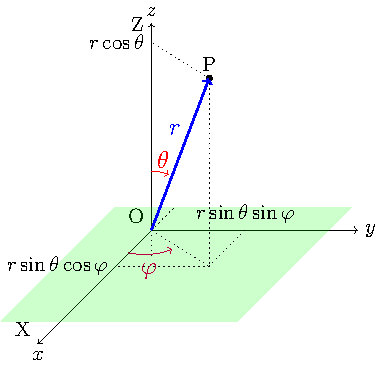
\includegraphics[width=6.2cm]{picture/vecter23.pdf}
 \caption{極座標系とDescartes座標系}
\label{fig:kyokuDeckankei}
 \end{center}
\end{figure}
\\
もし式(\ref{eq:kyokuDechenkan})に納得できないときは,
$\theta$がどんな角度だったかを思い出してほしい.
そうすればおそらく納得できるはずだ.
$\theta$がどんな角であるかを思い出せればPから$xy$平面に降ろした垂線の足と
原点との距離が$r \sin \theta$であることがわかる.
それさえわかればあとは自分でできるだろう.

さて,ここから基底同士の関係について考えてみよう.
そのためには,まず3次元極座標系における基底を定義しなくてはならない.

極座標系における座標が$(r, \, \theta, \, \phi)$であるような点Pについて考える.
OからPに向かう方向に長さ1のベクトルをとり,これを$\bm{e}_r$とする.
次に,極Oを中心とし,点Pを通り,かつ2直線OP,OZが張る平面に含まれるような円を考え,
その円の点Pにおける接線に平行な大きさ1のベクトルを$\theta$を測った向きにとり,
これを$\bm{e}_\theta$とする.
最後に,極Oを通り,$\bm{e}_\theta$に垂直な平面上に極Oを中心としてOPを半径とする円を考え,
その円の点Pにおける接線に平行な大きさ1のベクトルを$\varphi$を測った向きにとり,
これを$\bm{e}_\varphi$とする.
\begin{figure}[h]
 \begin{center}
 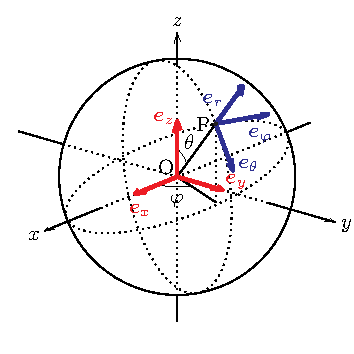
\includegraphics[width=7cm]{picture/vecter30.pdf}
 \caption{3次元極座標系における基底}
\label{fig:3dkyokukitei}
 \end{center}
\end{figure} \\
文章を読んで頭に思い浮かんだ図と図\ref{fig:3dkyokukitei}が一致するだろうか.
図\ref{fig:3dkyokukitei}から,$\bm{e}_r, \, \bm{e}_\theta, \, \bm{e}_\varphi$を
$\bm{e}_x, \, \bm{e}_y, \, \bm{e}_z$で表せば
\begin{align}
\begin{aligned}
\bm{e}_r & = & \sin \theta \cos \varphi \, \bm{e}_x & & + \sin \theta \sin \varphi \, \bm{e}_y &
& + \cos \theta \, \bm{e}_z & \\
\bm{e}_\theta & = & \cos \theta \cos \varphi \, \bm{e}_x & & + \cos \theta \sin \varphi \, \bm{e}_y & 
& -  \sin \theta \,  \bm{e}_z & \\
\bm{e}_\varphi & = & - \sin \varphi \, \bm{e}_x & & + \cos \varphi \, \bm{e}_y &
\label{eq:kyokuDeckitei}
\end{aligned}
\end{align}
となることがわかる.わかるといって理解できれば苦労しないので,
式(\ref{eq:kyokuDeckitei})に関しては少しばかり解説を入れておこう.
といっても,やることは2次元のときとそれほど大きく変わるわけではない.

$\bm{e}_r$について考える.図中の点P($r, \, \theta , \, \varphi$)と同じ方向に大きさ1だけ進むことを考えればよい.
簡単のため,$\bm{e}_r$の始点は極Oにあるとしておこう.
こういうことを考えるとき,3次元空間をある平面に正射影した図というのは非常に役に立つ.
正射影というと偉そうに聞こえるが,要は上から見るとか横から見るとかそういうことである.
\footnote{空間に存在する図形$S$と平面$\pi$について,$S$から$\pi$に降ろした垂線の足全体の集合を
$S$の$\pi$への正射影と呼ぶ.また,$S$の$\pi$への正射影を考えることを
$S$を$\pi$に正射影するという.}\index[widx]{せいしゃえい@正射影|textbf}
\begin{figure}[h]
 \begin{minipage}{0.5\hsize}
  \begin{center}
   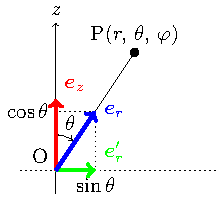
\includegraphics[width=5cm]{picture/vecter24}
  \end{center}
 \caption{3次元空間の直線OPと$z$軸を含む平面への正射影}
 \label{fig:z-OP}
\end{minipage}
\begin{minipage}{0.5\hsize}
  \begin{center}
   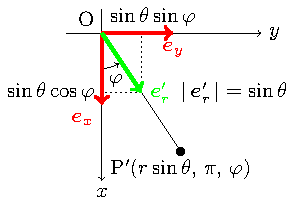
\includegraphics[width=6cm]{picture/vecter25}
  \end{center}
 \caption{3次元空間の$xy$平面への正射影}
 \label{fig:3dxy}
\end{minipage}
\end{figure} \\
まず,図\ref{fig:z-OP}を見てほしい.この図は3次元空間を直線OPと$z$軸を含む平面に正射影した図である.
$\bm{e}_r$はこの平面に含まれるベクトルである.
$\bm{e}_r$を$\bm{e}_z$と$\bm{e}_z$に垂直で,その終点が$\bm{e}_r$の終点から極Oを通り,
$z$軸に垂直な直線に降ろした垂線の足に一致するようなベクトル$\bm{e}'_r$とに分解する.
三角関数の定義から,$\bm{e}_r = \cos \theta \, \bm{e}_z + \bm{e}'_r $
が成り立つことはすぐにわかる.そして,$| \, \bm{e}'_r \, | = \sin \theta$が成り立つこともわかる.
そして,$\bm{e}'_r$は$xy$平面に含まれるベクトルなので,
$\bm{e}'_r$は$\bm{e}_x, \, \bm{e}_y$を用いて表せるはずだ.
そこで,3次元空間を$xy$平面に正射影したのが図\ref{fig:3dxy}である.
$\bm{e}_r$を$xy$平面に正射影すると$\bm{e}'_r$が得られる.
$\bm{e}'_r$の大きさは$\sin \theta$であり,従って$\bm{e}'_r$の始点を極Oに固定し,
極Oと$\bm{e}'_r$の終点から$x$軸に降ろした垂線の足までの距離は$\sin \theta \cos \varphi$となり,
そして極Oと$\bm{e}'_r$の終点から
$y$軸に降ろした垂線の足までの距離は$\sin \theta \sin \varphi$となる.
以上の考察により,$\bm{e}'_r = \sin \theta \cos \varphi \, \bm{e}_x 
+ \sin \theta \sin \varphi \, \bm{e}_y$が成り立ち,
従って$\bm{e}_r = \sin \theta \cos \varphi \, \bm{e}_x + \sin \theta \sin \varphi \, \bm{e}_y 
+ \cos \theta \, \bm{e}_z$が成り立つことがわかる.

次に,$\bm{e}_\theta$について考えよう.
これも正射影した図を見ながら考えることにする.
\begin{figure}[h]
 \begin{minipage}{0.5\hsize}
  \begin{center}
   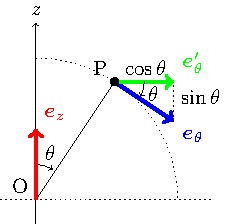
\includegraphics[width=4cm]{picture/vecter26}
  \end{center}
 \caption{3次元空間の直線OPと$z$軸を含む平面への正射影}
 \label{fig:z-OP-theta}
\end{minipage}
\begin{minipage}{0.5\hsize}
  \begin{center}
   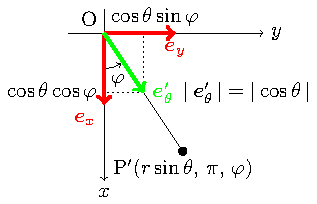
\includegraphics[width=6cm]{picture/vecter27}
  \end{center}
 \caption{3次元空間の$xy$平面への正射影}
 \label{fig:3dxy-theta}
\end{minipage}
\end{figure} \\
まず見るべきは図\ref{fig:z-OP-theta}である.
この図は3次元空間を直線OPと$z$軸を含む平面に正射影した図である.
$\bm{e}_r$のときと同じように$\bm{e}_\theta$もこの平面に含まれるベクトルである.
$\bm{e}_\theta$の始点を点Pに固定し,点Pを始点とし,$\bm{e}_\theta$の終点から
点Pを通り,$z$軸に垂直な直線に降ろした垂線の足を終点とするようなベクトルを$\bm{e}'_\theta$とする.
すると$\bm{e}_\theta$と$\bm{e}'_\theta$のなす角は$\theta$である.
このことは中学生でもわかることであるから省略させてもらおう.
このことから,$| \, \bm{e}'_\theta \, | = | \cos \theta \, |$となり,
\footnote{$\sin \theta$は$- \pi < \theta \leq \pi $の範囲では負にはならないが,
$\cos \theta$はそうはいかないので絶対値をつけている.
これ以外の``大きさ''や``距離''に関してはそういう配慮はしていない.}
$\bm{e}_\theta$は$\bm{e}_\theta = - \sin \bm{e}_z + \bm{e}'_\theta$と表せることがわかる.
$\bm{e}'_\theta$は$\bm{e}_r$のときと同じように考えて,図\ref{fig:3dxy-theta}から
$\bm{e}'_\theta = \cos \theta \cos \varphi \, \bm{e}_x + \cos \theta \sin \varphi \, \bm{e}_y$
と表せる.$| \, \bm{e}'_\theta \, | = | \cos \theta \, |$である以外はさっきとまったく同じである.
以上の考察の末,$\bm{e}_\theta = \cos \theta \cos \varphi \, \bm{e}_x 
+ \cos \theta \sin \varphi \, \bm{e}_y - \sin \theta \, \bm{e}_z$と表せることがわかる.
少しばかりややこしいが決して難しいというわけでもない.

最後に残るは$\bm{e}_\varphi$である.(始点を$xy$平面のどこかにしてみれば)
$\bm{e}_\varphi$は$xy$平面に含まれるベクトルなので,
$\bm{e}_x$と$\bm{e}_y$のみで表せるはずである.
よって,3次元空間を$xy$平面に正射影すると,それは図\ref{fig:3dxy-varphi}のようになる.
\begin{figure}[h]
 \begin{center}
 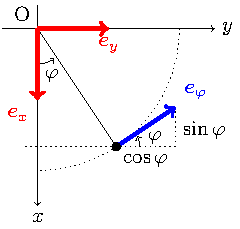
\includegraphics[width=4cm]{picture/vecter28.pdf}
 \caption{3次元空間の$xy$への正射影}
\label{fig:3dxy-varphi}
 \end{center}
\end{figure}
\\
$\bm{e}_\varphi$は原点を中心とし,OPを半径とする円の点Pにおける接線に平行なのであった.
図\ref{fig:3dxy-varphi}では,この円を回転し,さらに$\bm{e}_\varphi$を平行移動させて,
この円が$xy$平面上にあり,かつ$\bm{e}_\varphi$の始点が回転後の円の点Pに相当する点になるようにしてある.
$\bm{e}_\varphi$がOPと垂直であることや$\bm{e}_\varphi$を$\varphi$を測った向きに取ったことを加味すれば,
$\bm{e}_\varphi$と,$\bm{e}_\varphi$の始点を通って$y$軸に平行な直線のなす角は$\varphi$になり,
あとは$\bm{e}_r$や$\bm{e}_\theta$のときと同様に考えて
$\bm{e}_\varphi= - \sin \varphi \, \bm{e}_x + \cos \varphi \, \bm{e}_y$
となることがわかる.

以上で式(\ref{eq:kyokuDeckitei})は理解できたことになる.
実はもっと簡単にこの式を導く方法があるのだが,
それはまた後にしておこう.

なお,この基底$\Set{ \bm{e}_r , \, \bm{e}_\theta , \, \bm{e}_\varphi}$は
基底を構成するベクトルが互いに直交し,かつすべてのベクトルの大きさが1である.
このことは図からも明らかであるし,式(\ref{eq:kyokuDeckitei})
を用いて直接計算することもできる.
いちいち解説する必要もないだろう.

\subsubsection{円筒座標系}
3次元極座標系において,2次元極座標系を3次元極座標系に拡張するために用いたのは
新たに追加した始線と動径のなす角であった.
ここでは,別のアプローチをしてみよう.

極Oと始線OXをとり,さらに極Oを通ってOXに垂直な半直線を引く.
ここまでは3次元極座標系のときと同じであるが,
ここではこの直線に$z$軸という名前を付けよう.
そして,空間にある点Pに対し,Pと$z$軸との距離を$r$,
Pから$z$軸に降ろした垂線の足から極Oまでの(向き付きの)距離を$z$,
さらに,極Oを通ってOZに垂直な平面を考え,
極Oと,点Pからその平面に降ろした垂線の足の2点を通る直線を引く.
その直線と半直線OXのなす角を$\theta$とする.
これを図示してみれば,図\ref{fig:entou}のようになる.
\begin{figure}[h]
 \begin{center}
 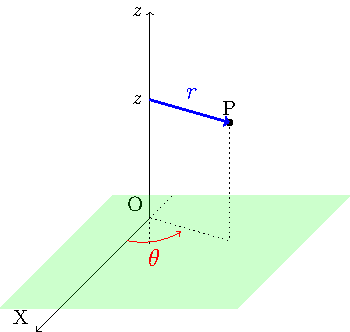
\includegraphics[width=5.2cm]{picture/vecter29.pdf}
 \caption{円筒座標系における座標の決定}
\label{fig:entou}
 \end{center}
\end{figure}


この$r, \, \theta, \, z$に対し,点Pの座標は$(r, \, \theta, \, z)$であると定めるのである.
極座標系のときと同じように,$z$軸上の点に対しては$\theta$の値を定めることはできないが,
やはりそういう細かいことは考えないことにする.
とにかく,こうして3次元空間にある点の座標を決定する規則,
すなわち座標系が導入できたわけである.

この座標系は,$z$軸の各点を中心とする無数の円が存在して,
$r$と$z$によって空間にある点がどの点にあるかを決定され,
$\theta$が点がその円上のどこにあるかを決定するようなイメージである.
$r$を固定して$z$と$\theta$を動かしてみれば,その軌跡は無限に長く伸びる円柱になる.
このことから,いま導入した座標系は
\emph{円筒座標系}\index[widx]{ざひょうけい@座標系!えんとう@円筒---}と呼ばれている.

さて,円筒座標系とDescartes座標系の関係について考える.
Descartes座標系における原点Oが円筒座標系における極Oに一致し,
さらにDescartes座標系における$x$軸,$y$軸が
それぞれ円筒座標系における半直線OXと$z$軸に一致するとしよう.
円筒座標系においてその座標が$(r, \, \theta, \, z)$であり,Descartes座標系における
座標が$(x, \, y, \, z)$であるような点において,以下に示すような関係式が成り立っている.
\begin{align}
\begin{aligned}
x & = r \cos \theta \\
y & = r \sin \theta \\
z & = z
\label{eq:entouDeczahyou}
\end{aligned}
\end{align}
式(\ref{eq:entouDeczahyou})に関してはもはや解説はいらないだろう.
2次元極座標系のときとまったく同様に考えておけばよい.

基底に関しても同様である.円筒座標系における座標が$(r, \, \theta, \, z)$であるような点Pにおいて,
半直線OPと同じ方向に大きさ1のベクトルをとり,これを$\bm{e}_r$とする.
さらに,Pから$z$軸に降ろした垂線の足を中心とし,半径$r$の円を考え,その円のPにおける接線に平行な
大きさが1のベクトルを$\theta$を測った向きにとり,これを$\bm{e}_\theta$とする.
最後に$z$軸と同じ向きに大きさ1のベクトルをとり,これを$\bm{e}_z$としておこう.
わざわざ図示しなくてもイメージできるはずだ.円筒座標系における基底は2次元極座標系のときの基底に
$\bm{e}_z$が生えたような様子になっている.
Descartes座標系での基底,つまり標準基底$\{ \, \bm{e}_x, \, \bm{e}_y, \, \bm{e}_z \, \} $との関係は
\begin{align}
\begin{aligned}
\bm{e}_r& = & \cos \theta \, \bm{e}_x & & + \sin \theta \, \bm{e}_y & \\
\bm{e}_\theta & = &  - \sin \theta \, \bm{e}_x & & + \cos \theta \, \bm{e}_y & \\
\bm{e}_z & = & & & & \; \; \; \;\;\;\; \bm{e}_z
\label{eq:entoukiteihenkan}
\end{aligned}
\end{align}
となる.この基底$\Set{ \bm{e}_r , \, \bm{e}_\theta , \, \bm{e}_z}$
を構成するベクトルは互いに直交するベクトルであり,かつすべてのベクトルの大きさが1である.
これも2次元極座標系のときとほとんど変わらない.
